% Nature Version of Record 2026-03-13, DOI 10.1038/s41586-025-09833-y.
% 非官方机器辅助中文译文; 图中 Lean 代码与证明状态保留原文, 不作为指令执行.
\originalchapter{基于强化学习的奥林匹克级形式化数学推理}\label{alphaproof-paper}
\begin{center}
\textbf{Olympiad-level formal mathematical reasoning with reinforcement learning}\par
Thomas Hubert、Rishi Mehta、Laurent Sartran 等, Google DeepMind\par
\textit{Nature} 651, 607--613 (2026)\par
正式记录版本: 2026 年 3 月 13 日; 初次在线发表: 2025 年 11 月 12 日\par
\url{https://doi.org/10.1038/s41586-025-09833-y}
\end{center}
\noindent\textbf{版本与许可.} 本译文以指定的正式 25 页 PDF 为对象, 不混用初始在线版的日期. 全部 39 位作者署名、机构与贡献见文末和 \texttt{metadata.json}. 原作按 CC BY 4.0 发布, 许可见 \url{https://creativecommons.org/licenses/by/4.0/}. 译者为 ai-self-study contributors, 采用机器辅助翻译和核对, 非 Google DeepMind 或 Nature 官方译本. 修改包括中文翻译、重新排版、图中文字对应说明和独立标识的译注; 作者数字、公式、代码、证明状态及各图署名保留. 译文与改编部分同样按 CC BY 4.0 提供.

\noindent\textbf{范围.} 完整转译正式文章的摘要、主文、全部方法、数学定义与搜索公式、实验、5 幅主图、主表 1、9 幅扩展数据图、2 张扩展数据表、参考信息和出版声明. 图中 Lean 代码、状态和高亮以原图保留, 自然语言题面、注释与图注另给完整中文对应. 独立的 Supplementary Information 和 Supplementary Data 1 附件不在此正式本体译文范围内; 对它们的引用原样保留, 不自动镜像不明许可的附件.

\begin{remark}
译注: 以下未标为译注的“我们”指原论文作者. Lean 检查形式命题的证明, 与自然语言题目是否被忠实形式化是不同问题. 作者的 IMO 成绩来自人工形式化、辅助答案生成、数日计算及 AlphaGeometry 2 的联合流程, 不应改写成模型在学生考试时限内独立完成整卷. 图中代码仅为原作数据; 本译文没有执行或重新验证这些 Lean 证明.
\end{remark}

\originalsection{摘要}\label{alphaproof-abstract}
人工智能 (AI) 的长期目标之一, 是建立能在广阔领域中进行复杂推理的系统. 数学以其无穷的概念和对严格证明的要求, 集中体现了这一任务. 近期 AI 系统往往依赖人类数据, 通常缺少保证正确性所需的形式验证. 相比之下, Lean\cite{alphaproof-ref1}等形式语言提供了能让推理落在可检验基础上的交互环境, 强化学习 (RL) 则提供在这些环境中学习的机制. 本文提出 AlphaProof, 一个受 AlphaZero\cite{alphaproof-ref2}启发的智能体, 通过在数百万个自动形式化的问题上进行 RL, 学习寻找形式证明. 对最困难的问题, 它使用测试时强化学习 (test-time RL, TTRL): 在推断阶段生成并学习数百万个相关问题变式, 实现深入的、针对特定问题的适应. AlphaProof 大幅提高历史数学竞赛题上的最先进结果. 在 2024 年国际数学奥林匹克 (IMO) 中, 以 AlphaProof 为核心推理引擎的 AI 系统解出了五道非几何题中的三道, 包括比赛最困难的一题. 与 AlphaGeometry 2\cite{alphaproof-ref3}结合, 在历时数日的计算条件下, 系统取得与银牌选手相当的分数. 据我们所知, 这是 AI 系统首次在该比赛达到任何奖牌等级的表现. 本工作表明, 大规模地从具有可验证依据的经验中学习, 可以产生具有复杂数学推理策略的智能体, 为复杂数学问题求解中的可靠 AI 工具铺路.

\originalsection{正文}\label{alphaproof-main}
AI 的重大挑战之一, 是开发能在复杂、开放式环境中有效推理并发现解答的智能体. 数学是科学理解的基础, 也是发展这些能力一个深刻而有意义的领域. 作为通向该目标的自然一步, 我们聚焦于顶尖数学竞赛中所需的推理能力. 这些竞赛本身虽不是开放式的, 但以要求创造性、多步骤深度推理的问题著称, 因而提供了衡量进展的关键标准化环境.

数学从欧几里得对几何的基础性公理化, 到符号代数记号的广泛采用, 历来不断走向更强的形式化. Lean 证明助手\cite{alphaproof-ref1}等现代计算机验证系统与 Mathlib\cite{alphaproof-ref4}等协作数学库, 是这一轨迹的逻辑延续, 使复杂数学能以机器可理解的格式表达. 在这些系统中, 形式证明不只是论证的序列, 而是一种称为“证明项”的特定数据结构, 编码了从公理到结论的完整逻辑论证. 虽然可以直接构造这些项, 用户通常交互式地应用称为 tactic 的动作来构建它们: 这些小程序操作当前证明状态 (假设与目标的集合), 每次推进一个逻辑步骤. Lean 内核检查生成的证明项是否为有效构造, 保证该过程的健全性. 这些系统提供两种革新能力: 严格、自动地验证每一步逻辑, 保证证明正确; 将数学转化为交互、可验证的领域, 使数学推理成为可以模拟、试验和学习的过程.

RL 是通过交互和经验学习的有力范式, 智能体通过试错优化行为, 达成指定目标. 在最优策略未知的复杂领域, 它已表现出很强的学习能力. 例如, AlphaZero 系列智能体在围棋、国际象棋和将棋\cite{alphaproof-ref2}等困难棋类游戏中达到超人类表现, 优化量子动力学\cite{alphaproof-ref5}, 并为排序\cite{alphaproof-ref6}和矩阵乘法\cite{alphaproof-ref7}等基础计算发现更高效的算法. 这些系统的力量来自: 能大规模与可验证环境交互, 利用有依据的试错反馈持续学习和细化策略. 因而, 将 RL 与形式系统结合, 是应对自动数学推理挑战特别有前景的方法.

虽然形式系统提供了可验证基础, 使用大量非形式化自然语言数学文本训练的大语言模型 (LLM), 也使 AI 数学推理取得显著进展. 这些模型能解答广泛的问题、生成类似人类的数学论述\cite{alphaproof-ref8,alphaproof-ref9,alphaproof-ref10}, 直接受益于文本中既有人类知识的规模与广度. 然而, 严格验证其推理正确性仍是活跃研究挑战. 目前所用技术包括与已知解答比较最终答案, 或借助无法完全信任的系统, 将生成的推理步骤与参考证明比较\cite{alphaproof-ref11,alphaproof-ref12}. 缺少正确性保证, 限制了它们在验证数学主张、或处理没有既有参考的问题时的可靠性. 相比之下, 形式系统自身的验证能力提供必要基础, 可以构建推理过程与输出可信的 AI 智能体, 即使探索超出既有人类证明和训练数据边界的内容.

AlphaProof 将形式系统的严格性与 RL 的经验学习结合, 在 Lean 定理证明环境内寻找证明, 并发展强大数学推理能力. 它显著提高历史顶尖数学竞赛题上的最先进结果; 特别是在 2024 年 IMO 中证明了五道问题中的三道. 虽然求解需要远超人类参赛者的计算时间, 这一成功仍展示了处理此前被认为超出自动系统能力的数学挑战的潜力.

\originalsection{AlphaProof}\label{alphaproof-system}
AlphaProof 是通过与基于 Lean 定理证明器的可验证环境交互、发现形式数学证明的 RL 智能体. 它的架构、训练和推断结合了若干关键创新.

\noindent\textbf{Lean 强化学习环境.} 与文献\cite{alphaproof-ref13,alphaproof-ref14}相似, 我们将 Lean 中交互证明过程建模为序贯决策问题, 这是 RL 任务的标准表述. 为将我们的形式 RL 任务与 Lean 证明助手本身区分, 把这个具体建模称为“Lean 环境”. 每个待证数学命题构成一个不同问题实例. 下面用状态、动作、奖励和回报等标准 RL 术语定义环境.

任一时间步 $t$, 状态 $s_t$ 是 Lean 证明器的逻辑状态, 包括已经建立的假设和未完成目标. 智能体将它观测为 Lean tactic 状态 (原文图 1a 左). 智能体以文本字符串提出动作 $a_t$, 即一个 Lean tactic. 环境尝试执行该 tactic, 更新假设和目标, 转移到新状态 (原文图 1a 右). 每个回合从新问题命题开始, 成功找到证明或超时则结束. 每次应用 tactic 给奖励 $r_t=-1$, 激励智能体寻找短证明. 从状态 $s_t$ 起的回报 $G_t$, 是直到终止的奖励之和. 关键是, 对分解成多个必须全部解决的独立子目标的证明状态, 回报定义为这些子目标回报的最小值, 即最长证明分支对应的回报, 而非较自然的各子目标回报之和. 完整 RL 建模及价值函数定义见“方法”.

\begin{center}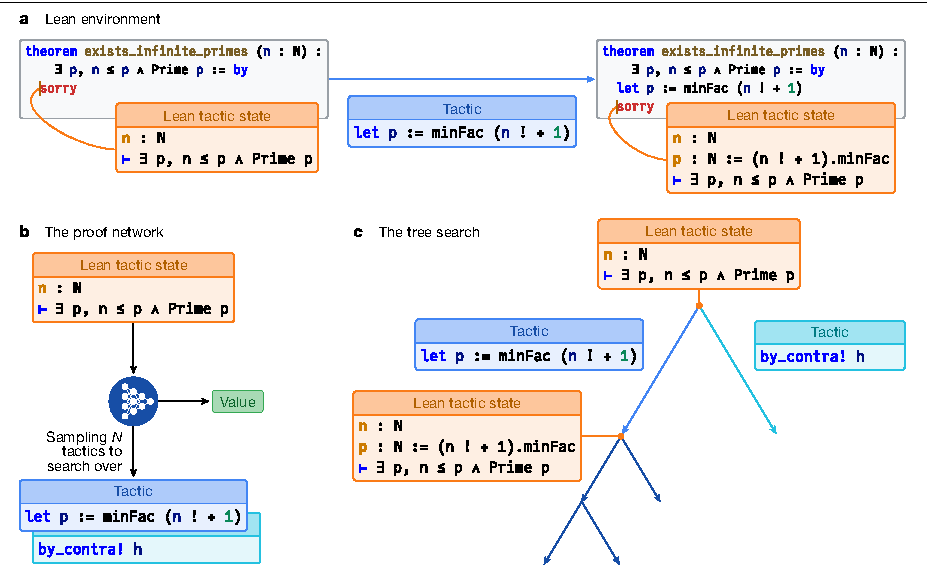
\includegraphics[width=\linewidth]{../papers/translations/alphaproof/assets/fig1.pdf}\end{center}
\phantomsection
\noindent\textbf{原文图 1. AlphaProof 的核心推理组成.}\paperlabel{1}{alphaproof-fig1}
a, 证明每一步所在的 Lean 环境. 智能体观测初始 Lean tactic 状态 (左), 描述待证定理. \texttt{sorry} 是 Lean 中表示证明未完成的占位符. 对环境应用一个 tactic, 例如原图的 \texttt{let p := minFac (n! + 1)}, 得到新状态, 可能引入新假设或改变目标 (右框). b, 证明网络以当前状态为输入, 输出 $N$ 个值得尝试的 tactic 和一个估计证明难度的价值. c, 树搜索使用这些输出探索可能证明路径: 从初始状态 (根) 开始迭代扩树, 每节点调用网络 (b), 生成有潜力的 tactic 与当前状态价值估计. 在环境 (a) 应用 tactic (边), 得新证明状态 (子节点). 网络价值智能指导搜索, 将计算集中于最有潜力路径, 例如更深入探索左分支.

\noindent\textbf{图中文字对应.} Lean environment: Lean 环境; Lean tactic state: Lean tactic 状态; Tactic: tactic; The proof network: 证明网络; The tree search: 树搜索; Value: 价值; Sampling $N$ tactics to search over: 采样 $N$ 个 tactic 供搜索. 所有 Lean 代码、$n,p$ 类型与假设、目标符号、分支和状态均以原图保留. 图中命题是对自然数 $n$ 寻找不小于 $n$ 的素数 $p$; \texttt{minFac} 为原代码的最小素因子操作名.


\noindent\textbf{证明智能体.} AlphaProof 把深度神经网络与受 AlphaZero\cite{alphaproof-ref2}启发的强大搜索算法结合. 核心是证明网络, 一个 30 亿参数的编码器--解码器 Transformer\cite{alphaproof-ref15,alphaproof-ref16}. 它学习解释观测到的 Lean tactic 状态 (原文图 1b), 并生成两个输出: 建议下一步有潜力 tactic 的策略, 以及估计预期回报 $G_t$ 的价值函数 (定义如前节). 这些输出指导专门的树搜索, 执行 tactic 序列并评估后果 (原文图 1c). 为形式定理证明作出的关键适配, 包括类似文献\cite{alphaproof-ref17}的 AND--OR 树结构, 处理证明分解出的多个必须全部解决的独立子目标. 为管理巨大、开放式的可能 tactic 空间, AlphaProof 对动作采样\cite{alphaproof-ref18}, 并使用渐进采样\cite{alphaproof-ref19}, 在关键路径上探索更广的证明策略. 网络架构和树搜索算法的完整细节见“方法”.

\noindent\textbf{训练.} AlphaProof 主要通过多阶段训练发展能力. 首先, 证明网络在约 3000 亿 token 的代码和数学文本上预训练, 使用语言模型标准的下一 token 预测目标. 该阶段旨在使网络广泛理解逻辑结构、编程语法与数学语言, 为后续从远小于此的数据集的形式数据中有效学习奠定必要基础. 随后, 在从 Mathlib\cite{alphaproof-ref4}人工证明提取的约 300,000 个状态--tactic 对上进行监督微调. 这个阶段使证明网络理解 Lean 语法与内部状态、模仿专家 tactic, 并给出证明难度的初始估计.

中心学习阶段是受 AlphaZero 启发的主 RL 循环, AlphaProof 从自身生成的经验中学习. 与棋类不同, 证明任务没有一个普适初始状态, 能通过自我博弈推导所有其他状态. 因此, 要跨多样数学领域学习推理, 必须有庞大、多样的问题命题语料, 作为 RL 智能体不同的起点. 人类数学问题是自然来源, 但人工形式化为 Lean 的题目数量, 比自然语言题少许多个数量级. 为弥合差距, 我们开发自动形式化过程 (原文图 2a 左、扩展数据图 2), 使用基于 Gemini、经人工和合成数据微调并迭代改进的 LLM. 项目期间, 该模型将约 100 万自然语言问题自动形式化为约 8000 万形式 Lean 问题. 其规模远超其他可用数据集. 每个自动形式化命题无论是否忠实于原自然语言题, 都是 AlphaProof 可以尝试证明或反驳的有效形式问题, 因而都是有用训练实例.

\begin{center}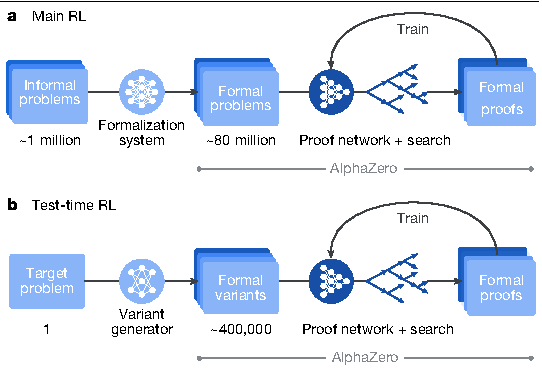
\includegraphics[width=\linewidth]{../papers/translations/alphaproof/assets/fig2.pdf}\end{center}
\phantomsection
\noindent\textbf{原文图 2. AlphaProof 的学习与适应过程.}\paperlabel{2}{alphaproof-fig2}
a, 主 RL 循环. 约 100 万非形式数学题先经形式化系统, 转为约 8000 万题的大规模形式数据集, 作为类似 AlphaZero 的 RL 课程. 证明网络结合树搜索, 在 Lean 环境生成形式证明与反证. 尝试获得的经验迭代训练、改进证明网络, 增强解答广泛问题的能力. b, TTRL 循环. 对一个具体困难形式问题, 变式生成器产生多样相关形式变式. 集中的、类似 AlphaZero 的 RL 再用证明网络与树搜索, 在这套定制变式课程上训练. 针对性学习使网络适应原题的结构和困难, 常能找到此前难以找到的形式证明. 可以同时处理多个目标. 图改编自文献\cite{alphaproof-ref28}, Google DeepMind.

\noindent\textbf{图中文字对应.} Main RL: 主强化学习; Test-time RL: 测试时强化学习; Informal problems: 非形式问题; Formalization system: 形式化系统; Formal problems: 形式问题; Proof network + search: 证明网络加搜索; Formal proofs: 形式证明; Train: 训练; Target problem: 目标问题; Variant generator: 变式生成器; Formal variants: 形式变式. 图内约 100 万、约 8000 万、1、约 400,000 等计数、AlphaZero 循环与箭头全保留原值.


任务匹配系统将自动形式化问题与自适应计算预算分配给分布式执行者, 随机让它们证明或反驳各命题. 执行者使用当前证明网络指导、在证明树上运行的树搜索算法, 于 Lean 环境生成尝试. 经 Lean 验证的结果, 无论证明、反证还是超时, 都提供有依据的反馈. 证明网络持续从成功证明和反驳尝试的经验改进 (原文图 2a 右), 细化策略以预测有效 tactic, 并调整价值以估计预期回报. 基于自身生成经验的持续改进, 使 AlphaProof 超越模仿既有证明, 发现解决困难问题所需的潜在复杂推理策略. 各训练阶段、自动形式化、任务匹配系统和计算预算汇总的完整细节见“方法”.

\noindent\textbf{推断.} 面对新问题, AlphaProof 利用两个互补的计算扩展机制, 都从主 RL 训练后的智能体初始化. 首先, 增加树搜索预算使证明路径探索更充分, 这是 AlphaZero 系列\cite{alphaproof-ref2}已证有效的技术. 其次, 对大量搜索仍可能不足的问题, 使用新的 TTRL 方法 (原文图 2b). TTRL 与主训练阶段使用相同的受 AlphaZero 启发的核心 RL 算法 (原文图 2a), 但不是从广泛的自动形式化问题课程学习, 而是聚焦为目标问题专门生成的合成变式课程, 例如简化题或推广题 (原文图 2b). 因而, TTRL 允许智能体投入大量资源学习问题专属策略, 往往解锁仅扩展树搜索仍难找到的解答. 完整细节见“方法”.

\originalsection{基准}\label{alphaproof-benchmarks}
我们在一套完整的形式数学基准上评估 AlphaProof, 全部由人工形式化为 Lean, 覆盖高中进阶、顶尖奥林匹克及大学水平的问题. 评估包括: (1) 公开 miniF2F 基准\cite{alphaproof-ref20}的修订版本, 对应高中数学竞赛; (2) formal-imo, 包含全部由内部专家形式化的历史 IMO 非几何题. 几何排除源于 Mathlib 对奥林匹克风格几何的具体限制, 见“方法”中“IMO 风格几何”; (3) 公开 Putnam 基准\cite{alphaproof-ref21}, 对应本科生普特南数学竞赛. Putnam 中自 1990 年起偶数年份的问题保留为独立留出测试集 PutnamBench-test. 所有训练阶段严格保持数据隔离, 确保评估一般化推理能力而非记忆; 数据整理和隔离细节见“方法”. 这些基准合起来构成标准化、多样且困难的测试平台, 评估 AlphaProof 的高级数学推理和求解能力.

\originalsection{主强化学习阶段的进展}\label{alphaproof-main-rl}
我们分析 AlphaProof 主 RL 阶段的表现. 该阶段训练约耗费 80,000 个张量处理器 (TPU) 日, 例如相当于 4,000 个 TPU 使用 20 日. AlphaProof 从自身生成经验学习, 尝试证明或反驳自动形式化数据集的数百万问题. 训练中, 成功证明或反驳的比例持续增加, 只剩一部分数据未判定, 展示对训练课程的掌握 (原文图 3a). 这种能力稳健推广到未见问题: 留出基准 miniF2F-valid、formal-imo、PutnamBench-test 的解题率持续改善, 从初始监督微调模型 (原文图 3b 的 0 TPU 日点) 发展到远超其他证明器的最终表现. 主 RL 阶段也显著提高寻找证明的效率. 随训练推进, 达到某个解题率所需的树搜索模拟显著减少 (原文图 3c), 表明网络成为更强指导者, 内化了有效证明策略. 这展示了如何将大量 RL 训练计算成本转为推断效率, 产生更强、更高效的智能体.

\begin{center}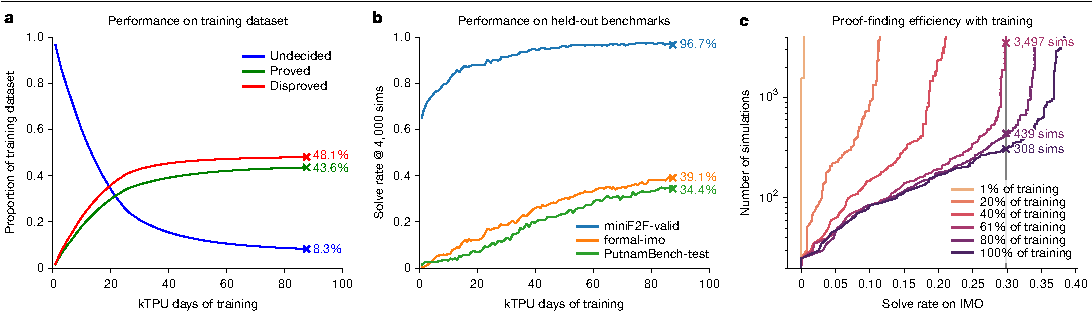
\includegraphics[width=\linewidth]{../papers/translations/alphaproof/assets/fig3.pdf}\end{center}
\phantomsection
\noindent\textbf{原文图 3. AlphaProof 在主 RL 中的学习进程.}\paperlabel{3}{alphaproof-fig3}
a, 训练集 (自动形式化问题) 上的表现演变. 曲线显示随 Google Cloud TPU v6e 计算增加, 起始实例中已证明 (绿)、已反驳 (红)、未判定 (蓝) 的比例. b, 训练期间留出集 miniF2F-valid、formal-imo、PutnamBench-test 在 4,000 次模拟 (sims) 的解题率. c, 主 RL 不同阶段达到历史 IMO 某个解题率所需的树搜索模拟数, 使用对数尺度. 每条曲线对应不同训练阶段检查点. 后期智能体不仅更强, 也更高效, 达到同一解题率所需搜索显著减少. 例如, 最终模型仅 300 次模拟就解约 $30\%$ 的问题, 早期模型即使更多搜索也无法达到该水平.

\noindent\textbf{图中文字对应.} Performance on training dataset: 训练集表现; Proportion of training dataset: 训练集比例; Undecided、Proved、Disproved: 未判定、已证明、已反驳; kTPU days of training: 训练计算 (千 TPU 日); Performance on held-out benchmarks: 留出集表现; Solve rate @ 4,000 sims: 4,000 次模拟解题率; Proof-finding efficiency with training: 随训练改变的寻证效率; Number of simulations: 模拟次数; Solve rate on IMO: IMO 解题率. 1\%、20\%、40\%、61\%、80\%、100\% of training 分别为对应训练进度. 各标注百分数与模拟数均保持原值.


\originalsection{推断时的计算扩展}\label{alphaproof-inference-scaling}
主 RL 训练完成后, 可通过推断阶段分配更多计算资源, 进一步增强对未见问题的表现. 我们探索运行在不同时间尺度上的两个互补扩展机制 (原文图 4). 首先, 增加树搜索预算, 所有基准的解题率均显著提高 (原文图 4a). 智能体学得的搜索策略, 即使低预算也提供很强基线, 例如每题在 1 个 TPU 上用 2 分钟. 逐步将预算扩到若干 TPU 小时, 解题率持续提高. 例如, 搜索从 2 TPU 分钟扩至 12 TPU 小时, formal-imo 与 PutnamBench-test 解题率提高超过 10 个绝对百分点. PutnamBench-train 也表现出类似扩展性质, 见扩展数据表 2.

对大量树搜索仍未解决的问题, AlphaProof 用 TTRL 进行更深入的问题专属适应 (原文图 4b; 方法见“方法”). 这种方法带来快速初始增益: 前 50 TPU 日就解决许多新问题, 更长训练期间仍持续发现新解答. 持续学习使表现显著超过仅扩展树搜索: 相较 12 TPU 小时搜索, formal-imo 与 PutnamBench-test 都再增加 15 个绝对百分点 (原文图 4b、原文表 1). TTRL 自身效果也受变式质量和数量影响 (扩展数据图 3). 原文图 4 的两个横轴有不同尺度: 树搜索是 TPU 小时, TTRL 是数百 TPU 日, 突出了两种机制不同的计算投入和能力. TTRL 是处理最困难问题的有力机制. formal-imo 与 PutnamBench-test 按数学主题分解的树搜索和 TTRL 扩展结果, 见扩展数据图 4, 展示随计算增加而动态改善的情况.

\begin{center}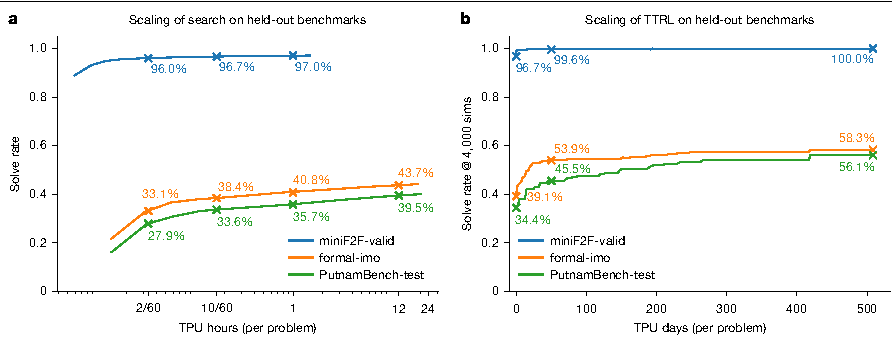
\includegraphics[width=\linewidth]{../papers/translations/alphaproof/assets/fig4.pdf}\end{center}
\phantomsection
\noindent\textbf{原文图 4. AlphaProof 表现随每题推断计算扩展.}\paperlabel{4}{alphaproof-fig4}
留出基准 miniF2F-valid、formal-imo、PutnamBench-test 的解题率. 两面板的“每题计算”均为评估 TPU 总计算除以基准题数的平均值. a, 解题率随树搜索每题计算增加的变化, 单位为 v6e TPU 小时, 对数尺度. 标出低预算, 如每题 $2/60$ TPU 小时即 1 个 TPU 用 2 分钟, 及更高预算的解题率. b, TTRL 扩展. 解题率随每目标题 TTRL 训练计算增加的变化, 单位为 v6e TPU 日, 线性尺度. 标出初步计算投入, 如 50 TPU 日或每题 50 个 TPU 用 1 日, 及 TTRL 结束的表现, 以 4,000 次模拟评估. 两面板横轴单位与尺度不同: 对数 TPU 小时与线性 TPU 日.

\noindent\textbf{图中文字对应.} Scaling of search on held-out benchmarks: 留出集上搜索扩展; Scaling of TTRL on held-out benchmarks: 留出集上 TTRL 扩展; Solve rate: 解题率; Solve rate @ 4,000 sims: 4,000 次模拟解题率; TPU hours (per problem)、TPU days (per problem): 每题 TPU 小时、每题 TPU 日. 坐标刻度、各曲线、标记与全部标注数字均保留.


\originalsection{最终基准评估}\label{alphaproof-final-evaluation}
完整的训练与推断扩展策略, 最终使 AlphaProof 在所有评估的形式数学基准上建立最先进表现 (原文表 1). 即使预算不高, 每题仅 2 TPU 分钟搜索, 它也在若干基准达到最先进结果 (原文图 4a、原文表 1). PutnamBench-test 的效率尤为突出, 大幅超过此前系统, 表明基础推理能力较强, 且在资源受限情境有效. 对最复杂问题的峰值表现, TTRL 至关重要, 以显著优势推进最先进水平 (原文图 4b). 它在所有基准带来全面增益 (原文表 1), miniF2F-valid 得满分 (扩展数据表 2), 测试集分数也接近满分. formal-imo 上, TTRL 在数论 ($75.7\%$) 和代数 ($72.6\%$) 特别强, 组合也取得进步 ($20.3\%$). PutnamBench-test 同样有全面增益. 主题细节见扩展数据图 3 和补充表 1; 补充信息也展示若干证明.

\Needspace{6\baselineskip}
\phantomsection
\noindent\textbf{原文表 1. AlphaProof 在形式数学基准上的表现.}\paperlabel{1}{alphaproof-table1}
\begin{longtable}{p{4.8cm}p{2.6cm}rrr}
\toprule
名称 & 每题计算预算 & \shortstack{miniF2F-test\\\cite{alphaproof-ref20}} & formal-imo & \shortstack{PutnamBench-test\\\cite{alphaproof-ref21}} \\
\midrule
\endfirsthead
\toprule
名称 & 每题计算预算 & \shortstack{miniF2F-test\\\cite{alphaproof-ref20}} & formal-imo & \shortstack{PutnamBench-test\\\cite{alphaproof-ref21}} \\
\midrule
\endhead
\multicolumn{5}{l}{\textbf{此前最先进结果 (IMO 2024 前)}} \\
GPT-F expert iteration\cite{alphaproof-ref24} & -- & 36.6\% & -- & -- \\
Hypertree proof search\cite{alphaproof-ref17} & -- & 41.0\% & -- & -- \\
InternLM2-Math-Plus-7B\cite{alphaproof-ref23} & -- & 43.4\% & -- & -- \\
\multicolumn{5}{l}{\textbf{此前最先进结果 (IMO 2024 后)}} \\
Kimina-Prover Preview\cite{alphaproof-ref25} & -- & 80.7\% & -- & 1.6\% \\
DeepSeek-Prover-V2\cite{alphaproof-ref26} & -- & 88.9\% & -- & 5.3\% \\
\multicolumn{5}{l}{\textbf{本工作}} \\
AlphaProof & 2 TPU 分钟 & 96.3\% & 33.2\% & 27.9\% \\
AlphaProof & 12 TPU 小时 & 97.7\% & 43.7\% & 39.4\% \\
AlphaProof 加 TTRL & 50 TPU 日 & 97.5\% & 53.9\% & 45.5\% \\
AlphaProof 加 TTRL & 500 TPU 日 & 99.6\% & 58.3\% & 56.1\% \\
\bottomrule
\end{longtable}
\noindent\textbf{原表注.} 每个其他系统使用其报告的最强结果, 对应最大计算预算, 与 AlphaProof 比较. “--” 表示计算预算或评估结果不可用. AlphaProof 的“每题计算预算”为原文图 4a 定义的平均计算成本, 只含推断预算, 不含主 RL 循环摊销成本. AlphaProof 的 miniF2F-test 使用修订版本, 见“方法”; 其他系统数值按各自论文和所用数据版本报告, 因而直接比较须考虑潜在数据差异并保持谨慎. PutnamBench-test 的此前工作分数, 按各系统公开报告的证明重新计算, 确保与本测试划分一致; 因此可能不同于那些系统在完整 PutnamBench 上报告的数字.


\originalsection{2024 年 IMO 的表现}\label{alphaproof-imo}
IMO 是世界最负盛名的大学前数学竞赛, 自 1959 年起每年举办. 各参赛国家派出至多六名通过严格国内竞赛选拔的优秀学生. 参赛者面对代数、组合、几何和数论的六道极具挑战的问题, 考查深入概念理解与创造性求解, 远超标准课程, 常需数小时专注思考. 获得 IMO 奖牌是重要荣誉, 常成为后来优秀数学家职业早期的标志.

为评估对未见竞赛的能力, 我们把 AlphaProof 用于 2024 年 IMO, 作为完整求解流程的核心推理引擎. 这一版本开发至 2024 年 7 月, 使用与前述相似的训练和推断方法. 因 Mathlib 对奥林匹克风格几何的具体限制 (见“方法”), 几何题 P4 交由专用 AlphaGeometry 2\cite{alphaproof-ref3}处理. 其余五道非几何题, 代数 P1、P6, 数论 P2, 组合 P3、P5, 在题目公布后立即由专家人工形式化为 Lean, 见“IMO 2024 评估协议与方法”.

P1、P2、P5、P6 等题需要先确定答案, 例如“找出所有函数……”, 再构造证明. 对这些题, 查询公开 Gemini 1.5 Pro 模型\cite{alphaproof-ref22}, 启用 Python 工具并给出一组人工少样本示例, 生成数百个候选答案. 对所有适用题, 它成功猜到了正确答案. AlphaProof 随后迅速反驳绝大部分错误候选, 展示高效率, 筛出正确候选作完整证明尝试. 借助 TTRL, 它为全部代数和数论题 P1、P2、P6 找到形式证明, 见扩展数据图 7--9. 每个解答都需要 2--3 日 TTRL, 表明推断阶段进行了大量问题专属适应. 两道组合题 P3、P5 仍未被系统解决.

联合系统由 AlphaProof 解决 P1、P2、P6, AlphaGeometry 2 解决 P4, 共解六题中的四题. 总分 28/42 (见“讨论与结论”), 进入官方比赛银牌区间, 比金牌线低一分 (原文图 5). 虽然 AlphaProof 解答的数日计算远超人类考生时间限制, 仍须注意, 此前最先进 AI 通常只能解历史 IMO 最简单题中的一小部分\cite{alphaproof-ref13,alphaproof-ref17,alphaproof-ref23}. AlphaProof 解出现场 IMO 三题, 包括仅五名人类考生解出的 2024 年最难 P6, 因而展示 AI 数学推理潜力的深刻进步, 即使应用于以困难、需要新见解著称的问题也是如此.

\begin{center}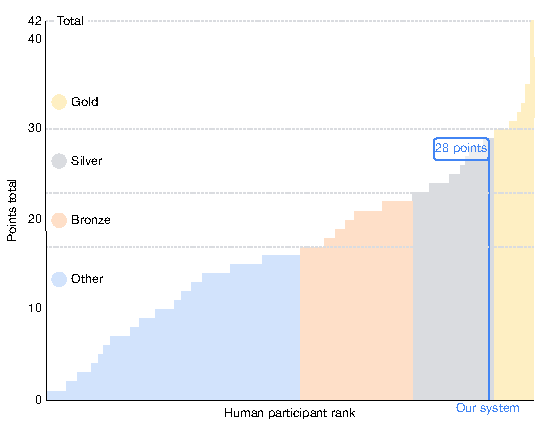
\includegraphics[width=0.75\linewidth]{../papers/translations/alphaproof/assets/fig5.pdf}\end{center}
\phantomsection
\noindent\textbf{原文图 5. 联合 AI 系统在 IMO 2024 的表现.}\paperlabel{5}{alphaproof-fig5}
联合系统得 28 分, AlphaProof 解三题 P1、P2、P6, AlphaGeometry 2\cite{alphaproof-ref3}解一题 P4. 相较人类参赛者\cite{alphaproof-ref27}, 该表现处于银牌区间. 图示官方金、银、铜牌分界. 图转载自文献\cite{alphaproof-ref28}, Google DeepMind.

\noindent\textbf{图中文字对应.} Total: 总分; Points total: 总得分; Gold、Silver、Bronze、Other: 金牌、银牌、铜牌、其他; Human participant rank: 人类参赛者排名; Our system: 我们的系统; 28 points: 28 分. 图中 42 分上限、奖牌边界与排名分布均保持原值.


\originalsection{讨论与结论}\label{alphaproof-discussion}
我们提出 AlphaProof, 一个能在 Lean 定理证明器形式环境中证明复杂数学问题的 RL 智能体. 它结合受 AlphaZero 启发的学习框架、数百万自动形式化问题课程与基于变式生成的 TTRL, 展示强大自动数学推理能力. 结果显示, 它在多样形式数学基准上显著推进最先进水平, 包括历史 IMO 与 Putnam 竞赛衍生基准. 2024 年 IMO 尤其展示了系统能力: 在完整求解流程中, AlphaProof 解出三道代数和数论题, 包括最难 P6; AlphaGeometry 2 解出几何题. 联合表现为解六题中的四题, 达到 2024 年 IMO 银牌选手相同分数. 据我们所知, 这是 AI 首次在 IMO 达到任何奖牌等级的里程碑, 为大规模从有依据、可验证经验中学习所涌现的复杂推理能力提供有力证据.

尽管结果是重要进展, 仍有局限和未来发展方向. 开源预训练基础模型如今已可取得, 但 AlphaProof 所需的专门学习阶段, 涉及的领域专属训练规模可能超出多数学术研究组能力. 此外, TTRL 解最困难题所需的数日推断虽然有效, 也说明需要更高效推断策略. 未来进步可能来自持续算法和工程改进、更先进自动形式化及更优化的 TTRL 策略.

当前成功主要限于高中进阶和本科竞赛数学. 这些问题虽极难, 但使用已知、固定的数学概念库, 主题也有一定一致性. TTRL 在该环境非常有效; 理解其推广性, 是把这些能力扩展到研究数学前沿的重要下一步之一. 这一转变尤其困难, 因为需要超越单纯解题、进入理论构建: 持续用新概念扩充数学库. 让 AI 理解数学品味、趣味或美, 最终仍是引人入胜的开放研究问题.

本工作的巨大计算需求, 提出可及性与开放研究生态未来的重要问题. 我们相信, 最合适的定位是基础性、探索路线的研究: 展示某能力可实现, 往往需要较大投入, 后续才可优化并让更多人使用. 为使工作成为社区催化剂而非壁垒, 我们采取了提供交互探索工具等具体措施. 未来研究关键方向是显著提高算法效率, 明确降低入门计算门槛, 使这些技术能成为整个数学界的协作工具. 尽管存在上述挑战, 我们预期持续发展, 特别是解决计算与范围局限, 将使 AlphaProof 成为人类研究者探索数学及其他科学前沿时越来越有价值的合作伙伴.

\originalsection{方法: 相关工作}\label{alphaproof-methods-related}
\noindent\textbf{交互式定理证明.} 本研究立足于交互式定理证明领域. 人类利用 Isabelle\cite{alphaproof-ref29}、HOL Light\cite{alphaproof-ref30}、Rocq\cite{alphaproof-ref31}、Lean\cite{alphaproof-ref1}等证明助手, 形式化定理并构造可验证证明. 这些工具促成四色定理的形式验证\cite{alphaproof-ref32}、CompCert C 编译器\cite{alphaproof-ref33}等关键软件的验证等重要成就. 但这类成功通常需要领域专家大量工作. AlphaProof 希望通过自动化定理形式化和证明的某些环节, 缓解瓶颈, 减少所需劳动和专业知识.

\noindent\textbf{定理证明中的机器学习.} 机器学习与定理证明的交叉领域已取得重要进展, 尤其是 LLM\cite{alphaproof-ref34,alphaproof-ref35,alphaproof-ref36}出现, 以及 MiniF2F\cite{alphaproof-ref20}、ProofNet\cite{alphaproof-ref37}、PutnamBench\cite{alphaproof-ref21}、LISA\cite{alphaproof-ref38}、HOList\cite{alphaproof-ref39}等形式数学基准可用之后. 本工作建立在这些进展上.

证明器对正确证明给出的自动反馈, 对大规模机器学习用于定理证明至关重要. 早期研究\cite{alphaproof-ref13,alphaproof-ref24,alphaproof-ref40,alphaproof-ref41}探索自动定理证明的生成式语言建模, 从人工证明学习, 并结合专家迭代或 RL. 同期, 若干研究\cite{alphaproof-ref14,alphaproof-ref42,alphaproof-ref43,alphaproof-ref44}关注 tactic 预测与前提选择的联合训练. 不同于逐步及搜索方法, Baldur\cite{alphaproof-ref45}率先使用 LLM 一次生成完整证明. 文献\cite{alphaproof-ref46}提出用非形式证明指导形式证明的“草稿、提纲与证明”方法; 子目标分解工作\cite{alphaproof-ref47}进一步扩展该路线. 神经定理证明还探索了更复杂搜索, 如 HyperTree Proof Search\cite{alphaproof-ref17}及蒙特卡洛树搜索变体\cite{alphaproof-ref48,alphaproof-ref49}. 最近, Kimina\cite{alphaproof-ref25}与 DeepSeek-Prover\cite{alphaproof-ref26}探索用 LLM 交错生成自然语言解释和形式证明.

\noindent\textbf{数学的自动形式化.} 弥合人工数学与形式证明器差距的关键组成是自动形式化, 即自动将自然语言数学命题译成形式证明或形式命题. 进展包括早期工作\cite{alphaproof-ref50,alphaproof-ref51}, 以及较近的基于 LLM 的方法\cite{alphaproof-ref52,alphaproof-ref53,alphaproof-ref54}. 后续研究用合成数据微调 LLM, 增强自动形式化\cite{alphaproof-ref49,alphaproof-ref55,alphaproof-ref56}; 更近的工作关注其评估\cite{alphaproof-ref57,alphaproof-ref58}. 我们开发自动形式化专门模型, 为证明智能体生成数百万形式命题, 扩展这些研究方向.

\noindent\textbf{LLM 推理.} 除专门证明器外, LLM 推理领域也有巨大进展. 思维链提示\cite{alphaproof-ref59}及常与规划结合的 RL, 显著增强了 LLM 推理, 尤其数学和编程任务\cite{alphaproof-ref60}. 最近, OpenAI O1\cite{alphaproof-ref61}和 DeepSeek R1\cite{alphaproof-ref9}展示扩展 RL 对 LLM 推理的有效性, 观察到训练时、测试时相对于计算的对数缩放. 这种方法在国际信息学奥林匹克达到相当于金牌的表现\cite{alphaproof-ref62}, 并在 AIME 表现强劲. 但 IMO 至今仍超出现有 LLM 的能力, 近期研究指出了它们有限的证明能力\cite{alphaproof-ref11,alphaproof-ref12}.

\noindent\textbf{TTRL.} 我们的方法扩展测试时计算缩放\cite{alphaproof-ref9,alphaproof-ref61,alphaproof-ref62,alphaproof-ref63}和适应\cite{alphaproof-ref64,alphaproof-ref65,alphaproof-ref66}趋势, 包括早期游戏中的 TTRL\cite{alphaproof-ref67,alphaproof-ref68}. 不同于这些方法, 也不同于同期用多数票奖励学习无标签非形式数学\cite{alphaproof-ref69}、或用数值验证学习递归简化积分变式\cite{alphaproof-ref70}的 TTRL, AlphaProof 的 TTRL (最初见文献\cite{alphaproof-ref28}) 专门处理顶尖形式数学问题, 尤其竞赛数学. 它在 Lean 中为困难 IMO、Putnam 级问题生成多样相关形式变式课程, 利用 Lean 严格验证指导学习, 最终在这个形式环境发现复杂、经过验证的证明.

\begin{remark}
译注: 上段“至今”“最近”均是原作研究时点的说法, 不是对读者阅读当天最新系统表现的重新判断.
\end{remark}

\originalsection{方法: 系统组成}\label{alphaproof-methods-system}
AlphaProof 是与基于 Lean 证明器\cite{alphaproof-ref1}的可验证环境交互、发现形式数学证明的 RL 智能体. 系统整合处理此复杂领域所需的核心技术: 定义定理证明任务的 RL 环境 (Lean 环境), 表示证明状态、建议证明后续步骤的深度网络 (证明网络), 面向形式证明的专门树搜索, 生成大规模训练问题集的翻译过程 (自动形式化), 发现一般证明策略的大规模 RL (主 RL), 以及处理困难实例的集中学习程序 (TTRL). 各组成详述如下.

\originalsection{方法: Lean 环境}\label{alphaproof-methods-lean}
\noindent\textbf{作为 RL 环境的形式数学.} 形式数学提供严格框架, 表达数学命题及其证明, 允许自动验证正确性. 我们使用 Lean 交互证明器\cite{alphaproof-ref1}, 它建立在称为归纳构造演算\cite{alphaproof-ref71}的依赖类型理论上. 在此范式中, 数学命题表示为类型, 证明对应于构造属于 (居留于) 该类型的项. 例如, 定理 $\forall P,Q,\ P\land Q\to Q\land P$ 可由函数项 \texttt{fun P Q }$\langle\texttt{hp, hq}\rangle\mapsto\langle\texttt{hq, hp}\rangle$ 证明, 该项属于对应类型. 最终由 Lean 可信内核检查正确性的, 正是这种“项模式”内容; Lean 也提供更高级“tactic 模式”, 使用户不必手工构造这些项. Tactic 通过操作含当前假设和目标的证明状态, 构造底层证明项. 例如, 上述定理也可用 \texttt{intro P Q h; simp [h]} 等 tactic 序列证明. 在 tactic 模式中, Lean 以 tactic 状态显示提供上下文, 呈现当前目标与关联假设 (原文图 1a、扩展数据图 1a). 正是这个模式被我们表述为 RL 环境 (扩展数据图 1b).

\noindent\textbf{状态 ($s_t$).} 状态表示证明尝试在时间步 $t$ 的完整 Lean 逻辑上下文, 包括全部活跃假设和剩余目标.

\noindent\textbf{观测.} 智能体观测到 Lean tactic 状态经过美化打印后的字符串表示.

\noindent\textbf{动作 ($a_t$).} 动作是一个用文本字符串表示的 Lean tactic.

\noindent\textbf{转移.} 将 $a_t$ 用于 $s_t$, 即让环境尝试执行 tactic. 若成功且有效 (见“tactic 验证和执行”), 得到假设和/或目标更新的新状态 $s_{t+1}$.

\noindent\textbf{回合.} 每回合从待证的新数学命题 (初始状态) 开始. 当找到初始命题的完整、经 Lean 验证的证明, 或预设计算预算耗尽时, 回合结束.

\noindent\textbf{奖励与目标.} 为激励发现最短证明, 每次应用 tactic 伴随 $r_t=-1$ 的奖励.

\noindent\textbf{回报定义.} 从 $s_t$ 起的 $G_t$ 为直到终止的奖励之和. 对分解为多个独立子目标的状态 (AND 节点, 见“与 Lean 对接”中“目标分解”), 回报以及价值函数目标, 定义为各子目标的最小回报, 即最长、最难证明分支对应的回报. 定义递归应用于这些多目标状态的祖先. 将所有子目标回报相加、从而最小化整个证明的 tactic 总数, 也是自然选择; 但取最小回报鼓励把目标分成难度平衡的子目标, 提供了有趣激励. 因而状态价值对应 $-T_{\rm steps}$, 其中 $T_{\rm steps}$ 是解决所有子目标所需证明最长分支中的 tactic 数.

\noindent\textbf{与 Lean 对接.} 为实现 RL, AlphaProof 与基于 Lean 4\cite{alphaproof-ref1}构建的定制环境交互. 它支持执行 tactic、处理证明状态、实现所需附加操作, 并为大规模树搜索作优化.

\noindent\textbf{Lean 核心与 Mathlib 集成.} 环境以 Lean 4 为基础证明助手, 加载广泛的 Mathlib\cite{alphaproof-ref4}, 提供大量数学定义、既有定理及高层 tactic, 例如线性算术求解器 \texttt{linarith}, 供智能体使用. 为支持遇到的具体领域 (如 IMO 风格问题) 的形式化, 并提供开发时主库尚缺的通用 tactic, 我们开发一组有限定制补充: 少量自定义定义、约 100 个初等定理以及针对常见符号操作的专门可复用 tactic, 如把 \texttt{(3/4).num} 简化为 3 的数值与列表简化. 补充旨在通用地处理常见模式或缺失低层基础设施. 其中许多后来被接纳进公开 Mathlib, 突出其广泛用途和与库发展目标的一致性.

\noindent\textbf{环境操作.} 为支持 AlphaProof 需求, 环境实现以下功能.

\noindent\textbf{并行执行与状态管理.} 环境设计为能在多线程同时管理和操作多个 Lean 证明状态, 允许树搜索并行模拟并高效批量查询网络. 实现了保存、恢复、唯一识别 tactic 状态的机制, 使树搜索可从任意此前访问状态继续.

\noindent\textbf{Tactic 验证与执行.} 网络提出文本 tactic 后, 环境尝试在当前状态执行. 成功应用不仅要求无错误执行, 还要求产生的证明项不使用不完整证明占位符 \texttt{sorry}, 且类型正确. 为评估类型正确性, 用一个私有 \texttt{internalSorry} 公理临时“关闭”未被该 tactic 直接处理的目标, 并捕捉 \texttt{have} 等 tactic 生成的中间主张. \texttt{private} 限制公理可见性, 避免在此 tactic 外使用. 最终健全性由 Lean 内核验证得到的闭合项保证, 见“与 Lean 对接”.

\noindent\textbf{目标分解 (AND 节点状态拆分).} 若 tactic 成功将当前目标分解为 $N>1$ 个独立子目标, 如把 $P\land Q$ 分为证 $P$ 与证 $Q$, 环境将当前 tactic 状态拆为 $N$ 个独立子状态. 每个子状态中, 除一个目标外全部赋予 \texttt{internalSorry}, 只留下一个开放目标. 这样每个子目标能在树搜索中当作独立问题, 构成搜索算法处理 AND 节点的基础, 见“树搜索算法”.

\noindent\textbf{反驳机制.} 为让智能体反驳命题, 即证明其否定, 环境提供将目标转为否定的操作. 它通过自定义 tactic 使用私有公理
\[
\texttt{internal\_true\_if\_false}: (\alpha\to\mathrm{False})\to\alpha.
\]
该 tactic 撤回全部局部假设, 应用公理并整理否定量词, 建立反驳原命题的新上下文: 它恰含此前完全量化目标的否定, 并以仍允许内核检查最终证明类型的方式实现, 见“与 Lean 对接”.

\noindent\textbf{性能与稳定性.} 为使环境在 RL 高吞吐需求下高效、稳健运行, 作了若干修改. 智能体常用的关键 Mathlib tactic, 如 \texttt{linarith}, 编译为 C 代码, 使某些 tactic 的执行 (生成证明项) 快六倍. 对单次 tactic 执行施加实际经过时间限制, 补充 Lean 内部按计算步计的 heartbeat 限制. 在关键代码路径更频繁调用监测资源消耗的 \texttt{checkSystem}, 提前安全终止耗时或耗资源的 tactic. 修改 Lean 的多精度整数库, 对数值大小设硬上限, 防止极大数引起失控计算.

\noindent\textbf{最终证明验证.} 为绝对保证正确性 (前提是 Lean 内核和所声明公理健全), AlphaProof 找到的每个证明或反证, 都经过最后独立验证. 在含完整定理命题和智能体证明的 \texttt{.lean} 文件上执行标准 Lean 命令行工具. 自定义命令也检查证明只依赖 Lean 内置三个常被接受的公理: 命题外延性、全局选择和商类型健全性.

\begin{remark}
译注: 搜索内部临时使用的 \texttt{internalSorry} 与 \texttt{internal\_true\_if\_false} 不应误读为最终证明获准依赖的额外公理. 原文明确另有完整证明的独立内核检查及公理依赖检查. 同时, 上述保证仍以形式命题、公理与内核健全性为前提, 不直接证明自然语言形式化的忠实性.
\end{remark}

\originalsection{方法: 证明智能体}\label{alphaproof-methods-agent}
\noindent\textbf{证明网络.} 网络是类似文献\cite{alphaproof-ref16}的 30 亿参数编码器--解码器 Transformer\cite{alphaproof-ref15}. 编码器接收美化打印的 Lean tactic 状态, 输出当前证明状态的潜在表示. 该表示送入两个不同的头: 解码器作为策略, 在推断时并行生成 $K$ 个 tactic; 价值头位于编码器之上. 与此前工作\cite{alphaproof-ref72}一致, 价值头将价值参数化为类别分布, 估计预期回报. 关键架构超参数汇总见补充表 2.

\noindent\textbf{树搜索算法.} 证明网络指导树搜索探索可能的证明构造. 搜索改编自 AlphaZero\cite{alphaproof-ref2}和 Sampled MuZero\cite{alphaproof-ref18}, 为形式证明作若干关键修改. 节点表示 Lean tactic 状态, 边表示该状态可用的 tactic (扩展数据图 1c). 每次搜索迭代有选择、扩展和反向回传三阶段. 关键超参数见补充表 3.

\noindent\textbf{标准树搜索框架. 选择.} 从根状态开始, 在每个状态 $s$ 递归选择使一个改编自文献\cite{alphaproof-ref2}的概率上置信树 (PUCT) 界\cite{alphaproof-ref73,alphaproof-ref74}最大的动作 $a$, 沿路径到叶节点:
\phantomsection\label{alphaproof-equ-a}
\[
Q(s,a)+c(s)\pi^{1/\tau}(a\mid s)
\frac{\sqrt{\sum_bN(s,b)}}{N(s,a)+1}.
\]
其中 $N(s,a)$ 是从 $s$ 访问 $a$ 的次数. 先验 $\pi^{1/\tau}(a\mid s)$ 来自网络策略输出, 经温度 $\tau$ 调整. 探索因子为
\phantomsection\label{alphaproof-equ-b}
\[
c(s)=c_{\rm init}+\log\left(\frac{N(s)+c_{\rm base}+1}{c_{\rm base}}\right).
\]
此前工作\cite{alphaproof-ref72}用状态 $s$ 全部子节点估计值的最大、最小值, 将 $Q(s,a)$ 归一化到 $[0,1]$; AlphaProof 则设置
\phantomsection\label{alphaproof-equ-c}
\[
Q(s,a)=\gamma^{-V(s,a)-1},
\]
其中 $\gamma$ 是折扣因子, $V(s,a)$ 是汇总搜索价值, 语义为解决当前目标剩余步骤数的负值. 对搜索中尚未访问的状态--动作对, 将 $V(s,a)$ 设为父节点网络预测 $V(s)$ 减一个固定惩罚.

\noindent\textbf{扩展.} 一次模拟到达尚未扩展的叶节点 $s_L$ 时, 从策略 $\pi(\cdot\mid s_L)$ 采样 $K$ 个 tactic. 在 Lean 环境验证每一个, 丢弃无效者; 将通往同一 Lean 状态的 tactic 合并 (允许对语法相同的假设改名或重排), 保留使一个关于字符串长度、执行时间线性依赖的成本函数最小者. 新扩展节点价值 $V(s_L)$ 由网络估计.

\noindent\textbf{反向回传.} 将扩展叶节点的价值估计沿选择路径回传, 更新所有经过的状态--动作对的 $N(s,a)$ 和 $V(s,a)$ 统计.

\noindent\textbf{AlphaProof 的关键适配. 渐进采样.} 为动态拓宽有潜力区域的搜索, 使用渐进采样. 若模拟路径上的节点 $s$ 满足 $n(s)\le C N(s)^\alpha$, 其中 $n(s)$ 是此前在 $s$ 采样 tactic 的次数、$N(s)$ 是总访问数, 再从 $\pi(\cdot\mid s)$ 采样 $K$ 个 tactic, 作为新边加到 $s$. 这使智能体能在关键路径上探索更广证明策略.

\noindent\textbf{多目标状态的 AND 节点.} 为管理多个独立子目标 (逻辑 AND 条件), 树搜索纳入概念上类似文献\cite{alphaproof-ref17}的 AND 节点. Tactic 将目标分解为多个独立子目标时引入 AND 节点, 见扩展数据图 1. AND 节点的动作对应选择一个子目标集中处理. 选择时, 仅考虑未证明子目标. 修改 PUCT, 优先处理被认为最困难的未证明子目标, 即具有最大 $V(s,a)$ 或最小 $Q(s,a)$ 的子目标. 实现方式是在标准 PUCT 中以 $1-Q(s,a)$ 替换 $Q(s,a)$. AND 节点 $s_{\rm AND}$ 对子目标 $a$ 的修改选择式为
\phantomsection\label{alphaproof-equ-d}
\[
\begin{aligned}
(1-Q(s_{\rm AND},a))
&+c_{\rm AND}c(s_{\rm AND})\pi(a\mid s_{\rm AND})
\frac{\sqrt{\sum_bN(s_{\rm AND},b)}}{N(s_{\rm AND},a)+1}.
\end{aligned}
\]
先验 $\pi(a\mid s_{\rm AND})$ 在全部子目标上均匀, $c_{\rm AND}$ 是额外乘子. 经 AND 节点回传时, 向上发送各子目标的最小 $V(s_{\rm AND},a)$, 与回报定义一致, 见“作为 RL 环境的形式数学”.

\begin{remark}
译注: 原文称最困难子目标有“最大 $V(s,a)$ 或最小 $Q(s,a)$”, 同时将 $V$ 定义为剩余步骤数的负值, 并给出上面的 $Q=\gamma^{-V-1}$ 及最小 $V$ 回传规则. 这些表述存在需要进一步澄清的符号关系; 本译文完整保留, 没有把 largest 静默改成 smallest. 四个显示搜索公式在原文 HTML 的定位 ID 为 Equa--Equd, 本文对应标签为 alphaproof-equ-a--d.
\end{remark}

\noindent\textbf{单次搜索.} 每次对初始问题的证明尝试, 执行一次搜索, 找到证明或反证、或模拟预算耗尽时结束. 不同于此前 AlphaZero 应用, AlphaProof 不承诺执行中间动作, 也不在一次尝试中从后续状态重新启动搜索. 这是因为形式系统中的定理证明类似完美模拟环境中的单人游戏. 智能体能在整个尝试期间保存并扩展一棵搜索树, 跨全部潜在证明路径全局分配计算资源, 无须先承诺某个中间步骤.

\originalsection{方法: 训练}\label{alphaproof-methods-training}
\noindent\textbf{预训练与监督微调.} RL 前, 证明网络通过多阶段训练初始化. 首先在约 3000 亿 token 的公开代码和数学文本上预训练, 使用下一 token 预测, 以 dropout 和掩码片段重建作正则化. 编码器处理约 12 万亿 token, 解码器重建约 3 万亿 token, 合计约遍历数据集 50 个 epoch. 这一阶段赋予策略头 (解码器) 对编程语法、逻辑结构与数学语言的广泛理解.

随后进行 SFT, 使用小得多但更专门的语料: 从 Mathlib\cite{alphaproof-ref4}人工证明提取约 300,000 个状态--tactic 对, tactic 约含 500 万 token. 该过程细化策略头的 Lean 专用 tactic 生成, 并根据 Mathlib 证明结构, 初始化价值头以估计证明剩余步数. 预训练和 SFT 超参数详见补充表 4.

\noindent\textbf{自动形式化.} 为向 RL 提供足够庞大、多样的课程, AlphaProof 依靠自动形式化, 将自然语言数学命题译为 Lean 形式语言 (扩展数据图 2), 从约 100 万条自然语言命题生成约 8000 万 Lean 问题.

\noindent\textbf{模型与训练数据.} 自动形式化系统基于专门微调的 Gemini 1.5 Pro, 训练三元组为自然语言题面、形式化思维链、Lean 形式命题. 初始数据约 2,500 个问题, 难度从代数预备到 IMO, 由专家人工形式化. 其中约 50 题, 专家还提供详述形式化步骤的思维链. 用专家标注示例提示公开 Gemini 1.5 Pro, 为既有翻译生成更多思维链, 将种子集扩至约 7,000 个三元组; 通过临时制定的格式规则检查识别并丢弃低质量合成思维链.

\noindent\textbf{迭代改进.} 为增强模型准确性, 使用类似 Self-Taught Reasoner (STaR)\cite{alphaproof-ref60}的策略. 对具有标准 (“golden”) Lean 形式化的问题子集, 当前微调模型反复生成思维链和 Lean 形式化, 过程见补充数据 1. 将生成命题与标准命题交给低计算预算 AlphaProof, 证明两者等价, 自动评估输出. 具体检查的 Lean 命题为
\[
\texttt{type\_of\% @generated = type\_of\% @golden}.
\]
获得等价的轨迹加入后续微调数据, 最终高质量三元组扩至约 70,000 个.

\noindent\textbf{评估与基准比较.} 通过 A/B 研究定期监测形式化模型: 在两个内部自然语言基准上比较基线与测试模型, 一个为 50 道代表性 IMO 题, 另一个为 50 道 Putnam 题 (补充表 5). 对每题, 两模型用标准化过程各生成一个形式化候选, 过程结合多数票、语法检查、循环一致性和 AlphaProof 快速反驳/证明尝试, 见补充数据 1. 随后由约三位内部 Lean 专家评估这些成对输出的逐项正确性与并列偏好.

2024 年 IMO 之前, 最终自动形式化过程在 50 道代表性 IMO 题上 pass@1 为 $60\%$, 代数 $81.3\%$、数论 $76.9\%$ 较强, 组合为较低的 $33.3\%$. 50 道 Putnam 题上 pass@1 为 $64\%$, 数论 $72.7\%$、代数 $61.9\%$、几何 $54.6\%$ 较强. 细节见扩展数据表 1.

\noindent\textbf{数据集生成.} 若干关键方法支持生成适合广泛数学问题形式化的训练数据. 对“找出所有 $n$……”等需要答案的题, 与问题一起收集合理答案, 在形式化时注入. 持续用改进流程重新处理来源题目, 扩充数据. 最后, 采样为每个自然语言问题生成多个不同形式翻译, 提高包含正确形式化的机会; 错误者常在主 RL 迅速判定, 有时本身也成为有趣问题. 最终获得有效 RL 训练所需的庞大多样数据集, 约 8000 万形式数学问题.

\noindent\textbf{主 RL.} 主 RL 从预训练与 SFT 初始化的网络继续训练. 架构包括集中任务匹配系统、分布式执行者和集中学习者. RL 共训练约 100 万步, 见补充表 6.

\noindent\textbf{起始状态数据集.} 课程主要是自动形式化生成的约 8000 万问题命题. 另补充小部分、约 3,500 个人工形式化问题, 来自 (1) miniF2F-curriculum\cite{alphaproof-ref24}; (2) 训练形式化模型时人工形式化的问题; (3) 我们的 Putnam 训练划分 PutnamBench-train, 由文献\cite{alphaproof-ref21}排除 PutnamBench-test 得到.

\noindent\textbf{任务匹配系统.} 它向可用执行者分配任务, 为每项任务从起始数据选择形式命题, 随机指定证明或反驳目标. 问题按最近 $N$ 次尝试结果确定的“趣味性”优先选择. 以下情况被认为很有趣: 尚未尝试; 尝试少于 \texttt{trust\_count}; 或次数超过 \texttt{trust\_count}, 但最近 $N$ 次有成功也有失败. 相反, 达到 \texttt{trust\_count} 次后始终未解, 或连续 \texttt{trust\_count\_proved} 次已证明、显示掌握的题, 优先级降低. 已成功反驳的命题不重试. 每次尝试的模拟预算自适应确定: 从基础值开始, 按该题最近 $N$ 次中的失败数乘法增加, 直到预定义上限, 从而给困难命题更多计算. 超参数见补充表 7.

\noindent\textbf{执行者生成经验.} 收到命题和预算后, 执行者在 Lean 环境交互, 用当前证明网络指导树搜索, 见“证明智能体”和“树搜索算法”. 不同于此前工作\cite{alphaproof-ref2}, 智能体从不承诺某个动作, 而是搜索至找到 Lean 验证的证明或反证, 或耗尽模拟预算. 将验证结果报给任务匹配系统, 更新问题统计. 搜索发现的证明、反证被提取并发送给学习者; 失败尝试被筛除, 不参与网络更新.

\noindent\textbf{学习者与网络更新.} 学习者持续以状态--tactic 对批量更新参数. 固定比例为 $10\%$ 来自 Mathlib SFT 数据, $90\%$ 来自保存执行者证明与反证的重放缓冲区. 策略头用交叉熵预测 tactic; 价值头预测当前证明 (子)目标所得回报. 经验生成和网络更新迭代进行, 逐步增强数学推理能力. 超参数见补充表 6.

\noindent\textbf{计算预算汇总.} 通用预训练之后的 AlphaProof 专门训练包含若干高计算阶段. Mathlib SFT 较便宜, 约 10 TPU 日. 后续投入很大: 整个项目生成约 8000 万问题课程的自动形式化, 共约 100,000 TPU 日, 例如相当于十次各使用 2,000 个 TPU、持续 5 日的运行. 从课程学习的主 RL 与之规模相近, 约 80,000 TPU 日, 例如 4,000 个 TPU 使用 20 日.

\originalsection{方法: 推断}\label{alphaproof-methods-inference}
主 RL 后, AlphaProof 具备对广泛数学问题寻找证明的一般能力. 推断时面对新、未见定理, 可用多种策略分配额外计算, 增强能力.

\noindent\textbf{扩展树搜索.} AlphaZero 系列\cite{alphaproof-ref2,alphaproof-ref72}推断增加计算的主要方法, 是扩大树搜索并运行多次独立尝试. 增加模拟次数, 使智能体细化网络最初建议的 tactic, 跨更多、更深推理路径整合信息, 探索其他证明序列. 搜索增强使 tactic 选择更强, 找到证明的概率更高. 多次独立尝试也提高概率, 通过并行化改善延迟. 原文图 4a、表 1 的结果展示, 将树搜索计算 (通常按计算量或实际经过时间计) 扩展, 能提高留出基准表现.

\noindent\textbf{使用 TTRL 扩展.} 对广泛树搜索仍难解决的题, AlphaProof 用 TTRL 进行更深的问题专属适应 (原文图 2b). 过程包含生成问题专属变式课程、在课程上集中 RL 两阶段.

\noindent\textbf{生成 TTRL 课程变式.} 对每个目标 Lean 实例 $T$, 首先生成专属合成变式课程. 使用 Gemini LLM\cite{alphaproof-ref22}, 以整理的 791 个问题--变式 Lean 对作为少样本提示. 这些示例展示, LLM 可模仿建立在经典策略\cite{alphaproof-ref75}及证明工程形式对应物上的启发式生成变式, 如简化\cite{alphaproof-ref76}、推广\cite{alphaproof-ref77}、提出引理\cite{alphaproof-ref78}、探索类比\cite{alphaproof-ref79}和从既有证明学习\cite{alphaproof-ref80}. 基于采样提示策略, LLM 生成单个候选或相关候选集合, 如问题分解、模拟证明步骤. 此外用程序生成变式, 系统覆盖局部变化, 例如系统改变 $T$ 的假设或目标. 所有候选经 Lean 语法正确性验证.

为丰富课程, 一个演化改进过程迭代扩充变式集合: 有潜力的已验证变式, 例如字符串与 $T$ 高度相似者, 递归作为进一步 LLM 生成的种子, 最多迭代 $N_{\rm evo}$ 次, 报告结果中 $N_{\rm evo}=15$. LLM 与程序生成、验证、演化改进的迭代, 再去重后, 为每个 $T$ 得到数十万独特、语法有效的 Lean 变式 $V_T$. 它们构成后续 RL 的局部、结构化课程, 过程详见补充数据 1, 样例见扩展数据图 5.

\noindent\textbf{集中 RL.} 生成变式后, AlphaProof 执行受 AlphaZero 启发的核心 RL, 从主 RL 通用模型初始化专门智能体. 与主 RL 的关键差别是课程: 不再是一般自动形式化命题, 而是目标 $T$ 及其语法生成变式 $V_T$. 框架可同时用于多个目标, 将所有变式纳入任务匹配系统共享起始集, 实现原文图 4b 中的并行多题 TTRL. 后续学习与主 RL 一致: 任务匹配系统协调分布式执行者, 反复证明或反驳问题, 见“主 RL”、补充表 7 的 TTRL 超参数. 成功证明或反证的状态--tactic 对经验, 用于更新专门证明网络, 见“主 RL”、补充表 6. 为优化计算预算, 目标 $T$ 一旦成功证明, 任务匹配系统就不再为 $T$ 及其 $V_T$ 分配新尝试, 因为主目标已完成. 问题专属适应使智能体细化已有策略, 可能发现解决目标的关键见解.

TTRL 因而允许推断时投入大量、有针对性的计算. 将完整 RL 机制策略性地重新用于特定问题适应, 使 AlphaProof 能解固定通用模型仅靠标准推断难解的定理. 系统生成、求解相关且常更简单的变式, 逐步走向复杂目标的解答, 正是波利亚\cite{alphaproof-ref75}著作强调的人类数学求解核心原则所启发的方法. 留出基准提升展示其效果, 见原文图 4b、表 1.

\originalsection{方法: 评估}\label{alphaproof-methods-evaluation}
我们使用覆盖高中进阶、顶尖奥林匹克和大学问题的完整形式数学基准评估 AlphaProof.

\noindent\textbf{标准基准.} formal-imo 包含全部由内部专家形式化的历史 IMO 非几何题, 排除几何的理由见“IMO 风格几何”. 它有 258 题: 代数 107、组合 77、数论 74, 有官方主题时使用官方分类, 否则由领域专家分类. 逐题表现见扩展数据图 6. 我们也评估内部修订的 miniF2F\cite{alphaproof-ref20}, 将 test 和 valid 均作为留出测试集. 修订处理原数据的形式化错误, 如可反驳命题、或假设自相矛盾的命题. 同时评估包含困难本科题的 Putnam 基准\cite{alphaproof-ref21}. 留出集 PutnamBench-test 含 1990 年起偶数年份的 189 题, 每题可有一个或多个主题. 最常见主题为代数 78、分析 57、数论 33、几何 20、线性代数 18. 项目中发现原 PutnamBench 的若干形式化错误, 随后在上游修订.

\noindent\textbf{数据隔离与推广.} 为严格评估推广能力, 我们精心管理各训练阶段数据隔离. 基础语言模型的初始预训练使用广泛网络语料, 可能偶然含某些历史题的自然语言讨论或解答, 但预训练流程明确排除所有 Lean 代码, 特别是评估基准对应的形式证明. SFT 仅训练 Mathlib, 它不含评估问题. 主 RL 只用自动形式化课程和人工补充题, 见“主 RL”. 关键是, 从自动形式化流程明确移除所有被判断与任一评估题过于相似的文档. 这一隔离协议旨在让表现反映学到的推理能力而非记忆.

\noindent\textbf{IMO 风格几何.} 开发时 Mathlib 高层几何库存在具体缺口, 如内切圆、全等, 因而在 Lean 中处理 IMO 平面几何困难, 许多题连陈述都不实际. 所以专门奥林匹克几何题, 如 IMO 2024 P4, 使用专为现代奥林匹克几何设计的 AlphaGeometry 2\cite{alphaproof-ref3}. AlphaProof 则使用 Mathlib 可用几何, 处理几何--组合混合 IMO 题及全部 PutnamBench 题, 后者纯平面几何较少.

\noindent\textbf{IMO 2024 评估协议与方法.} 为严格评估现场、分布外推广, 比赛遵循特定预定义协议. 事先与 Timothy Gowers 爵士教授和 Joseph Myers 博士约定, 由他们作为独立专家评委, 按官方 IMO 给分规则评估系统任何解答.

\noindent\textbf{赛前冻结.} IMO 2024 正式题目发布前, 主 RL 停止, 全部系统超参数冻结.

\noindent\textbf{问题形式化.} 公布后立即由专家人工将五道非几何题译为 Lean. 这一做法经指定 IMO 评委咨询后采用: 他们认为主要评估目标是系统解答已经形式陈述的问题的能力, 而非竞赛条件下从自然语言翻译题目的能力. 专家形式化也对应人类考生必要时可获得母语题目翻译的情形. P5 (组合) 尤其难以形式化, 专家最初尝试在第一日没有成功. 与人工工作并行, 我们作自动形式化侧面实验, 实际成功形式化 P1、P2、P6. 对“找出所有……”等需要答案的题, 形式化中答案部分用 \texttt{sorry} 占位, 系统负责生成候选, 见主文.

\noindent\textbf{答案猜测.} 生成过程专门优化为尽可能在大量候选中包含正确答案, 即对很大 $k$ 的 pass@k 优化, 即使会产生许多合理但错误候选. 我们生成 $k=500$ 个答案, 在所有适用题成功猜出正确者. AlphaProof 随后在高效筛选这些提议中至关重要: 低计算反驳模式下, 每候选树搜索最多 10 分钟, 它反驳了 Gemini 错误候选中 P1 的 $99\%$、P2 的 $98\%$、P6 的 $7\%$, 筛出有潜力者作完整证明.

\noindent\textbf{几何题.} 因“IMO 风格几何”说明的理由, P4 由 AlphaGeometry 2\cite{alphaproof-ref3}处理.

\noindent\textbf{验证与评判.} AlphaProof 产生的 P1、P2、P6 解答 (扩展数据图 7--9), 先由 Lean 内核验证正确, 再由 Timothy Gowers 爵士教授和 Joseph Myers 博士按官方 IMO 给分规则评判. 他们给每道已解决题满分.

\originalsection{扩展数据}\label{alphaproof-extended-data}
\begin{center}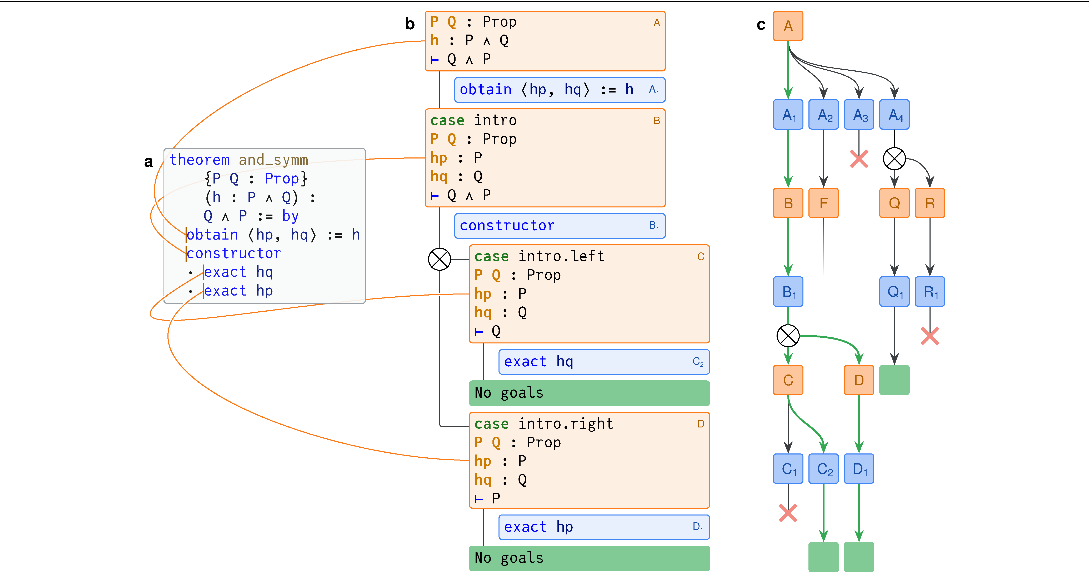
\includegraphics[width=\linewidth]{../papers/translations/alphaproof/assets/edfig1.pdf}\end{center}
\phantomsection
\noindent\textbf{扩展数据图 1. Lean tactic 环境及其树搜索建模.}\paperlabel{扩展数据 1}{alphaproof-edfig1}
a, Lean 编辑器环境, 光标位置关联 tactic 状态信息. b, 对应证明树, 通过动作 (tactic) 连接观测 (tactic 状态). $\otimes$ 表示有多个必须全部解决的子目标. c, 搜索树, 粗绿箭头高亮找到的成功证明.

\noindent\textbf{图中文字对应.} No goals: 无剩余目标. a 面板完整代码保持原样: 对命题 $P,Q$ 证明 $Q\land P$; 先从假设 $P\land Q$ 取出 \texttt{hp,hq}, 用 \texttt{constructor} 分开合取目标, 分别由 \texttt{exact hq}、\texttt{exact hp} 完成. b 的所有假设、目标、\texttt{case intro}、\texttt{case intro.left}、\texttt{case intro.right} 状态与 A--D 编号, c 的全部节点、失败叉号和 AND 符号均以原图保留.

\begin{center}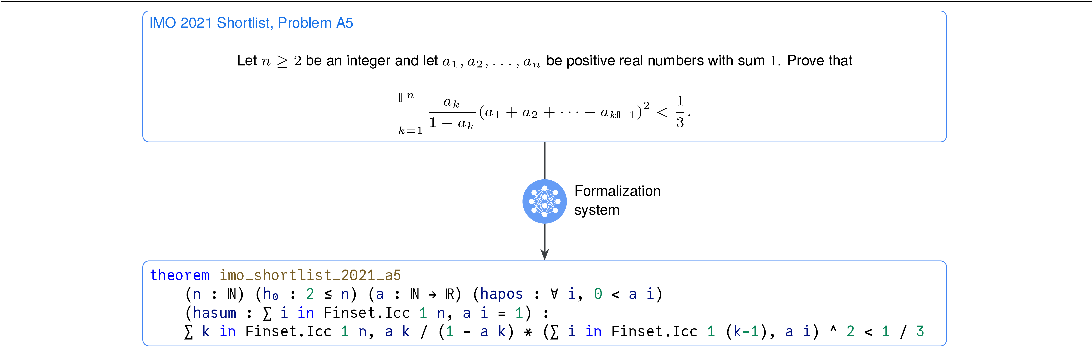
\includegraphics[width=\linewidth]{../papers/translations/alphaproof/assets/edfig2.pdf}\end{center}
\phantomsection
\noindent\textbf{扩展数据图 2. 自动形式化过程的一个例子.}\paperlabel{扩展数据 2}{alphaproof-edfig2}
原文图 2a 的形式化系统接收以 LaTeX 排版的自然语言题面, 输出有效 Lean 代码形式命题. 署名: Google DeepMind.

\noindent\textbf{图内题面完整中译.} IMO 2021 候选题, A5. 设整数 $n\ge2$, 正实数 $a_1,\ldots,a_n$ 的和为 1. 证明
\[
\sum_{k=1}^n\frac{a_k}{1-a_k}(a_1+a_2+\cdots+a_{k-1})^2<\frac13.
\]
Formalization system: 形式化系统. 下方完整 Lean 命题, 包括 $n$ 类型、$h_0$、$a$、\texttt{hapos}、\texttt{hasum}、有限集合求和上下界及目标不等式, 按原图保留.

\begin{center}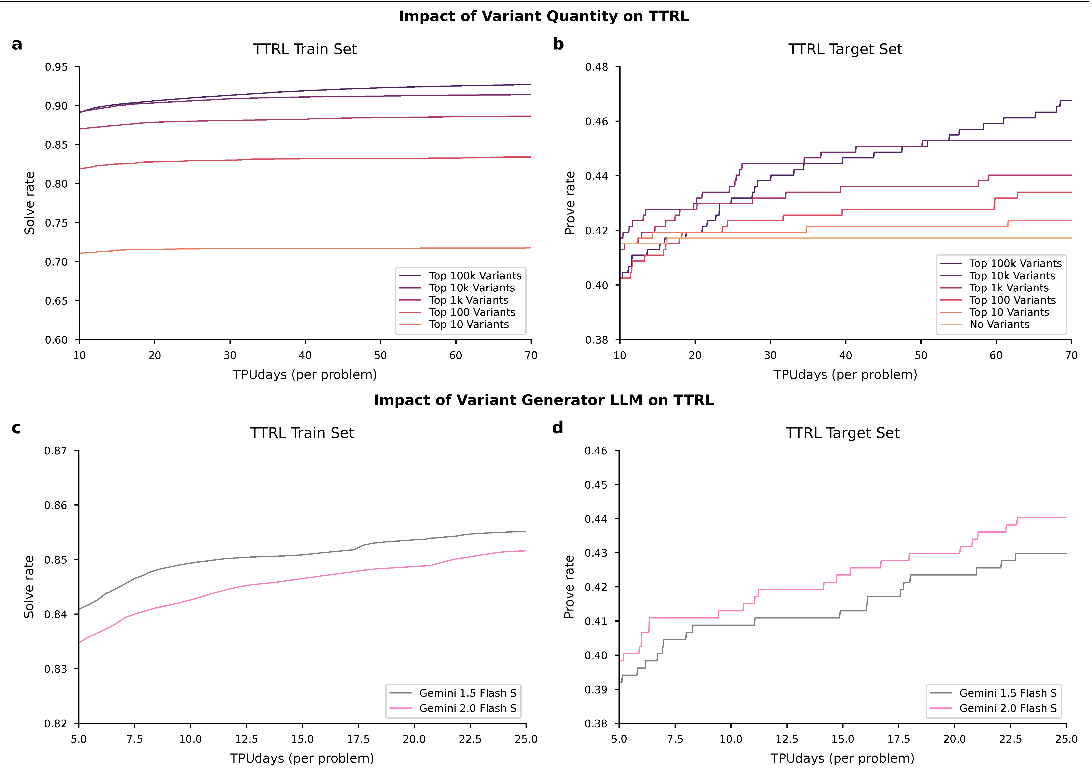
\includegraphics[width=\linewidth]{../papers/translations/alphaproof/assets/edfig3.pdf}\end{center}
\phantomsection
\noindent\textbf{扩展数据图 3. 改变合成变式数量及变式生成 LLM 的 TTRL 消融.}\paperlabel{扩展数据 3}{alphaproof-edfig3}
a, 增加课程变式数, 从 Top 10 到 Top 100k, 提高 TTRL 训练集内已解决变式比例. b, 更多合成变式持续提高目标题最终证明率, 展示更大问题专属变式集的显著益处. c, Gemini 1.5 Flash S (灰) 的训练变式解题率高于更强 Gemini 2.0 Flash S (粉), 提示后者变式可能构成更难课程. d, Gemini 2.0 Flash S 生成变式使目标题证明率显著更高, 说明该课程确实更有效.

\noindent\textbf{图中文字对应.} Impact of Variant Quantity on TTRL: 变式数量对 TTRL 的影响; Impact of Variant Generator LLM on TTRL: 变式生成 LLM 对 TTRL 的影响; TTRL Train Set: TTRL 训练集; TTRL Target Set: TTRL 目标集; Solve rate: 解题率; Prove rate: 证明率; TPUdays (per problem): 每题 TPU 日; Top 100k、Top 10k、Top 1k、Top 100、Top 10 Variants: 排名前 100,000、10,000、1,000、100、10 个变式; No Variants: 无变式. 模型名、曲线和全部坐标值保持原样.

\begin{center}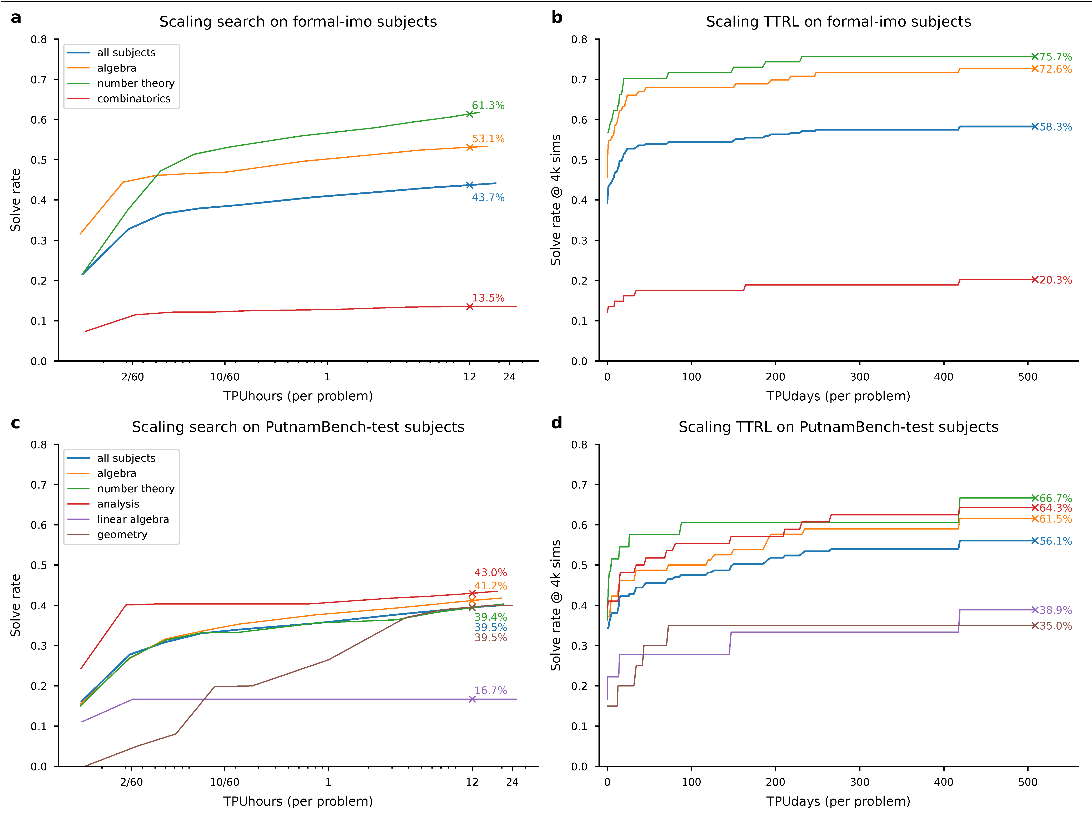
\includegraphics[width=\linewidth]{../papers/translations/alphaproof/assets/edfig4.pdf}\end{center}
\phantomsection
\noindent\textbf{扩展数据图 4. formal-imo 与 PutnamBench-test 按数学主题划分的推断扩展动态.}\paperlabel{扩展数据 4}{alphaproof-edfig4}
按主题细分两个基准的树搜索和 TTRL 解题率扩展. 粗蓝线为总体基准表现, 细线为具体主题表现.

\noindent\textbf{图中文字对应.} a、b 为 formal-imo 主题上的搜索、TTRL 扩展; c、d 为 PutnamBench-test 主题上的搜索、TTRL 扩展. All subjects: 全主题; algebra: 代数; number theory: 数论; combinatorics: 组合; analysis: 分析; linear algebra: 线性代数; geometry: 几何. Solve rate: 解题率; Solve rate @ 4k sims: 4,000 次模拟解题率; TPUhours (per problem)、TPUdays (per problem): 每题 TPU 小时、每题 TPU 日. 所有百分数、刻度及曲线原样保留.

\begin{center}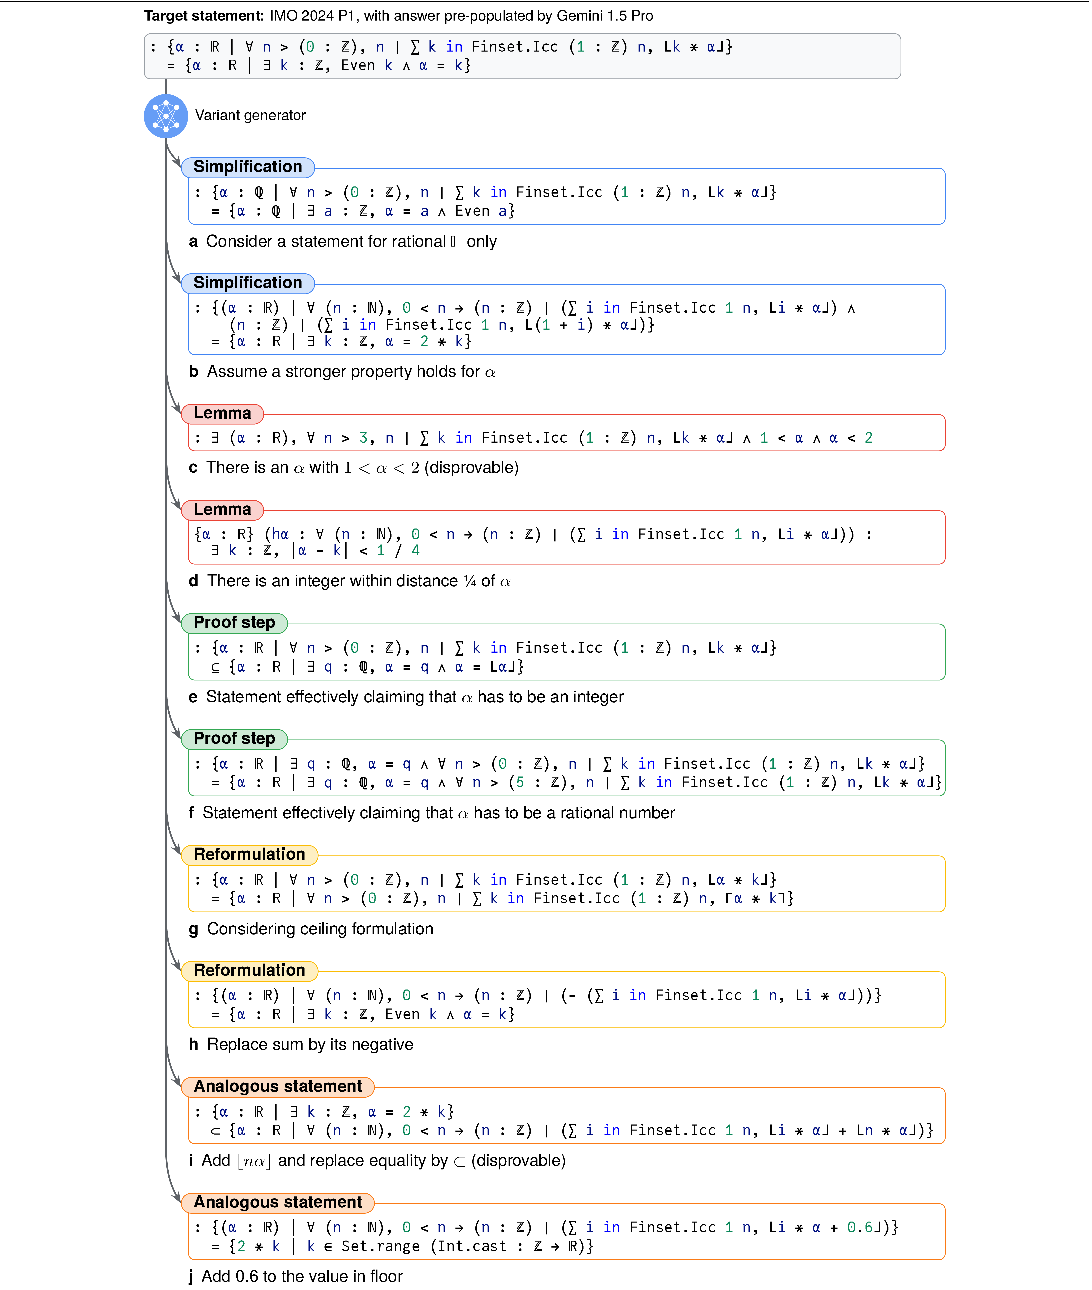
\includegraphics[width=\linewidth]{../papers/translations/alphaproof/assets/edfig5.pdf}\end{center}
\phantomsection
\noindent\textbf{扩展数据图 5. AlphaProof 为 IMO 2024 P1 自动生成的合成变式样例.}\paperlabel{扩展数据 5}{alphaproof-edfig5}
这些 Lean 变式在 TTRL 自动创建, 作者在此加标签和描述, 展示简化、提出引理、证明步骤、重新表述、探索类比等多样启发式. 处理这些变式帮助理解目标, 使证明智能体适应具体问题.

\noindent\textbf{图内文字完整中译.} Target statement: 目标命题, IMO 2024 P1, 答案由 Gemini 1.5 Pro 预先填入. Variant generator: 变式生成器. a, Simplification (简化): 只考虑有理数的命题. b, Simplification: 对 $\alpha$ 假设更强性质. c, Lemma (引理): 存在 $1<\alpha<2$ 的 $\alpha$, 此命题可反驳. d, Lemma: 在距 $\alpha$ 小于 $1/4$ 的范围有整数. e, Proof step (证明步骤): 实质声称 $\alpha$ 必须为整数的命题. f, Proof step: 实质声称 $\alpha$ 必须为有理数的命题. g, Reformulation (重新表述): 考虑上取整形式. h, Reformulation: 用和式的相反数替换和式. i, Analogous statement (类比命题): 加入 $\lceil n\alpha\rceil$ 并用整除替换, 该命题可反驳. j, Analogous statement: 对下取整中的值加 0.6. 目标和 a--j 每个变式的完整 Lean 代码、量词、数值、集合、有限求和、上下取整符号及颜色, 全部保持原图, 不将可反驳变式改成正确命题.

\begin{center}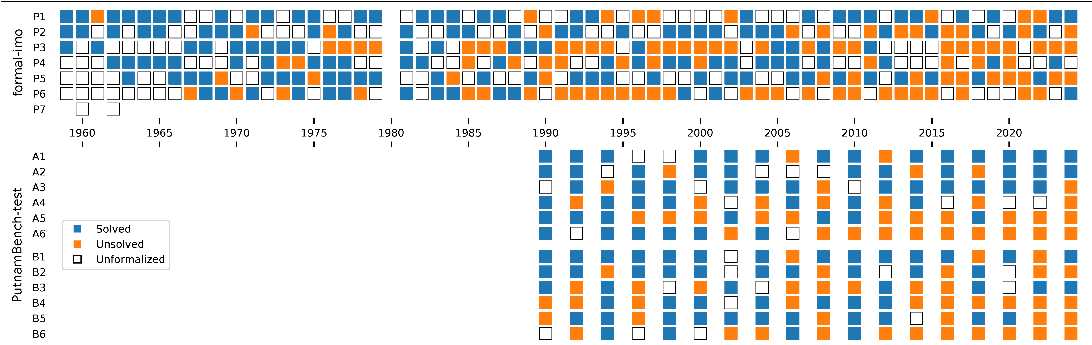
\includegraphics[width=\linewidth]{../papers/translations/alphaproof/assets/edfig6.pdf}\end{center}
\phantomsection
\noindent\textbf{扩展数据图 6. formal-imo 与 PutnamBench-test 在 TTRL 结束或主 RL 时解决的问题.}\paperlabel{扩展数据 6}{alphaproof-edfig6}
蓝为已解决, 橙为未解决, 白为未形式化. IMO 因政治原因在 1980 年未举行.

\noindent\textbf{图中文字对应.} Solved: 已解决; Unsolved: 未解决; Unformalized: 未形式化. 每个年份、题号 P1--P7、A1--A6、B1--B6 及对应颜色方格保持原样; 未形式化不同于尝试后未解.

\clearpage
\noindent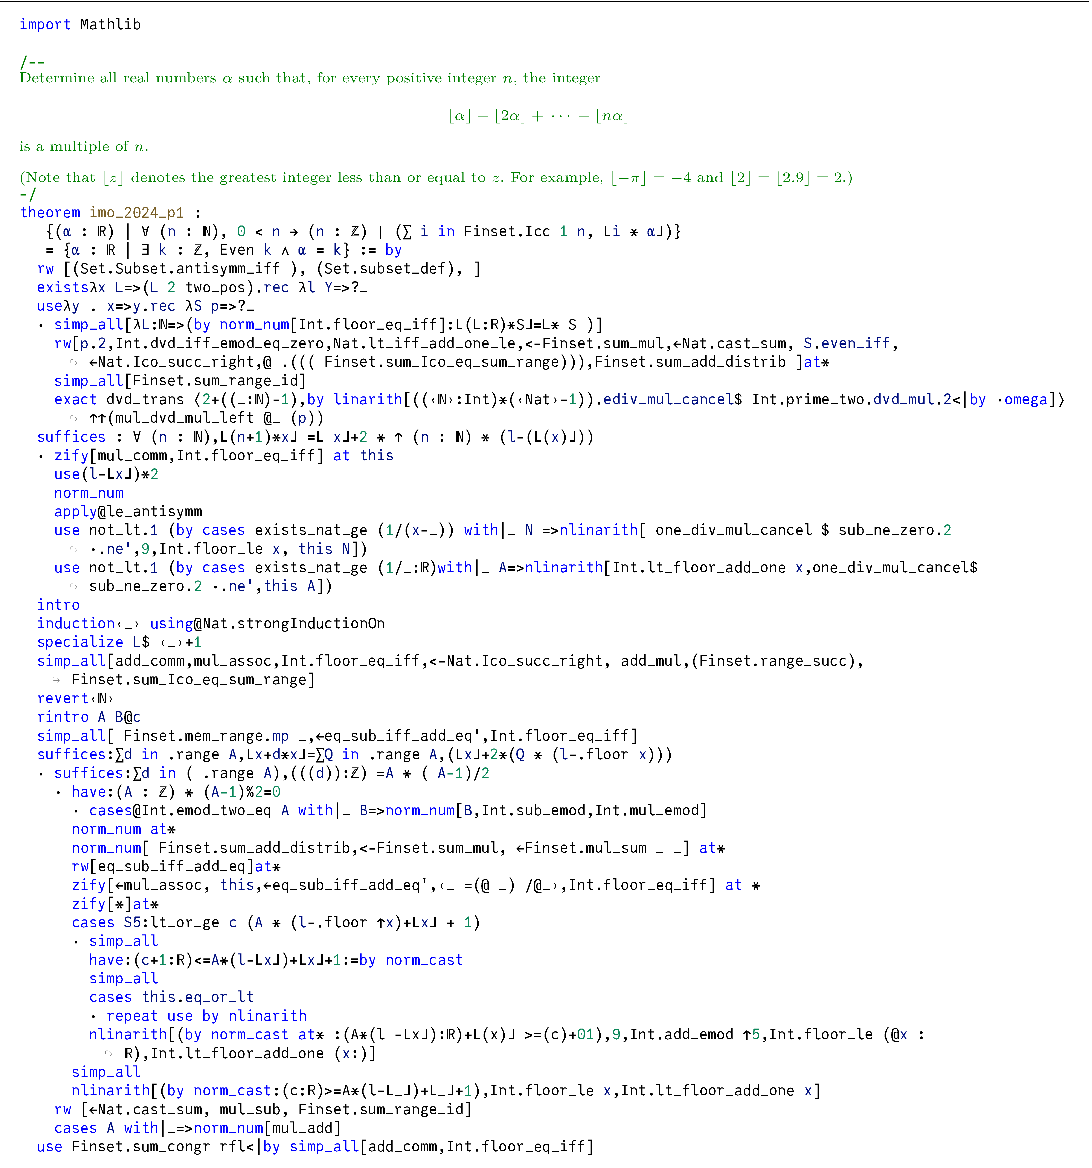
\includegraphics[width=\linewidth]{../papers/translations/alphaproof/assets/edfig7.pdf}\par
\phantomsection
\noindent\textbf{扩展数据图 7. AlphaProof 找到的 IMO 2024 P1 完整证明.}\paperlabel{扩展数据 7}{alphaproof-edfig7}
按第 6.4 节协议找到. 本图及扩展数据图 8、9 的交互版本见文献\cite{alphaproof-ref28}, 可查看全部中间 Lean 目标状态. 609 名学生中 413 人完整解出了此代数题\cite{alphaproof-ref27}. 图改编自文献\cite{alphaproof-ref28}.

\noindent\textbf{代码题面注释完整中译.} 求所有实数 $\alpha$, 使每个正整数 $n$ 都满足整数
\[
\lfloor\alpha\rfloor+\lfloor2\alpha\rfloor+\cdots+\lfloor n\alpha\rfloor
\]
是 $n$ 的倍数. $\lfloor z\rfloor$ 表示不大于 $z$ 的最大整数, 例如 $\lfloor-\pi\rfloor=-4$, $\lfloor2\rfloor=\lfloor2.9\rfloor=2$. 原图从 \texttt{import Mathlib} 到最后一个 tactic 的完整代码、全部量词、证明分支和形式解集均保留; 形式命题的解集表述为偶整数. 此处仅翻译注释, 不把代码改为另一份证明, 也不声称本译文重新编译验证过它.

\clearpage
\noindent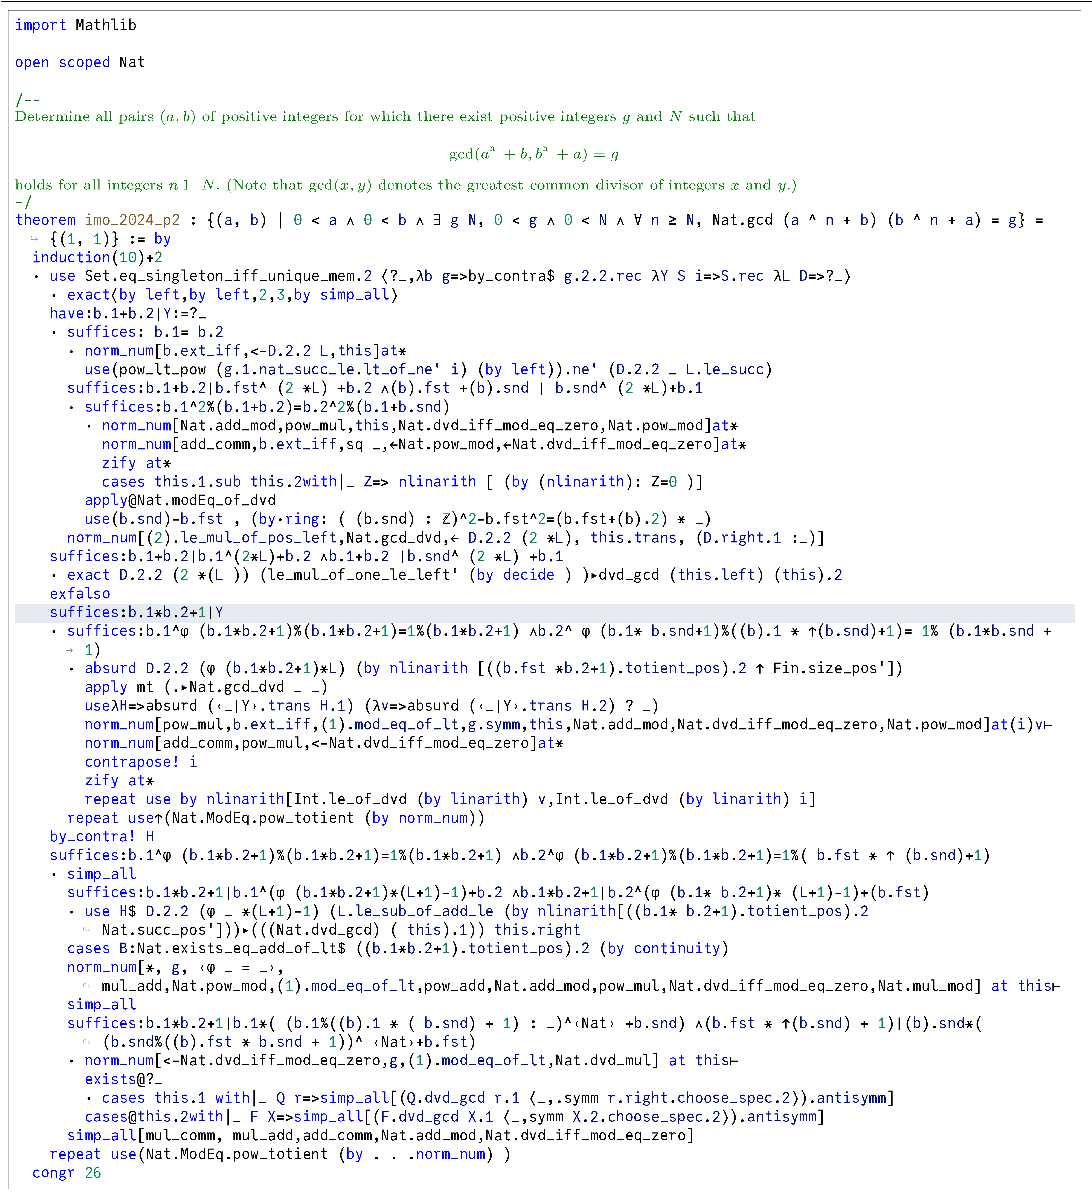
\includegraphics[width=\linewidth]{../papers/translations/alphaproof/assets/edfig8.pdf}\par
\phantomsection
\noindent\textbf{扩展数据图 8. AlphaProof 找到的 IMO 2024 P2 完整证明.}\paperlabel{扩展数据 8}{alphaproof-edfig8}
按第 6.4 节协议找到. 证明关键是考虑 $ab+1$ 的性质, 例如它整除 $g$, 在高亮行可见. 609 名学生中 156 人完整解出了此数论题\cite{alphaproof-ref27}. 图改编自文献\cite{alphaproof-ref28}.

\noindent\textbf{代码题面注释完整中译.} 求全部正整数对 $(a,b)$, 使存在正整数 $g,N$, 对所有整数 $n\ge N$ 均有
\[
\gcd(a^n+b,b^n+a)=g.
\]
$\gcd(x,y)$ 表示整数 $x,y$ 的最大公因数. 原图完整保留 \texttt{import Mathlib}、\texttt{open scoped Nat}、解集 $\{(1,1)\}$ 的形式定理、全部代码与高亮行.

\begin{remark}
译注: 原 PDF 英文题面注释中 $n$ 与 $N$ 之间的比较符号显示不完整. 紧接的 Lean 正式命题明确为 $\forall n\ge N$; 上文据该代码转录为 $n\ge N$. 原图仍按原件保留, 没有修补图像或声称图内字形已恢复.
\end{remark}

\clearpage
\noindent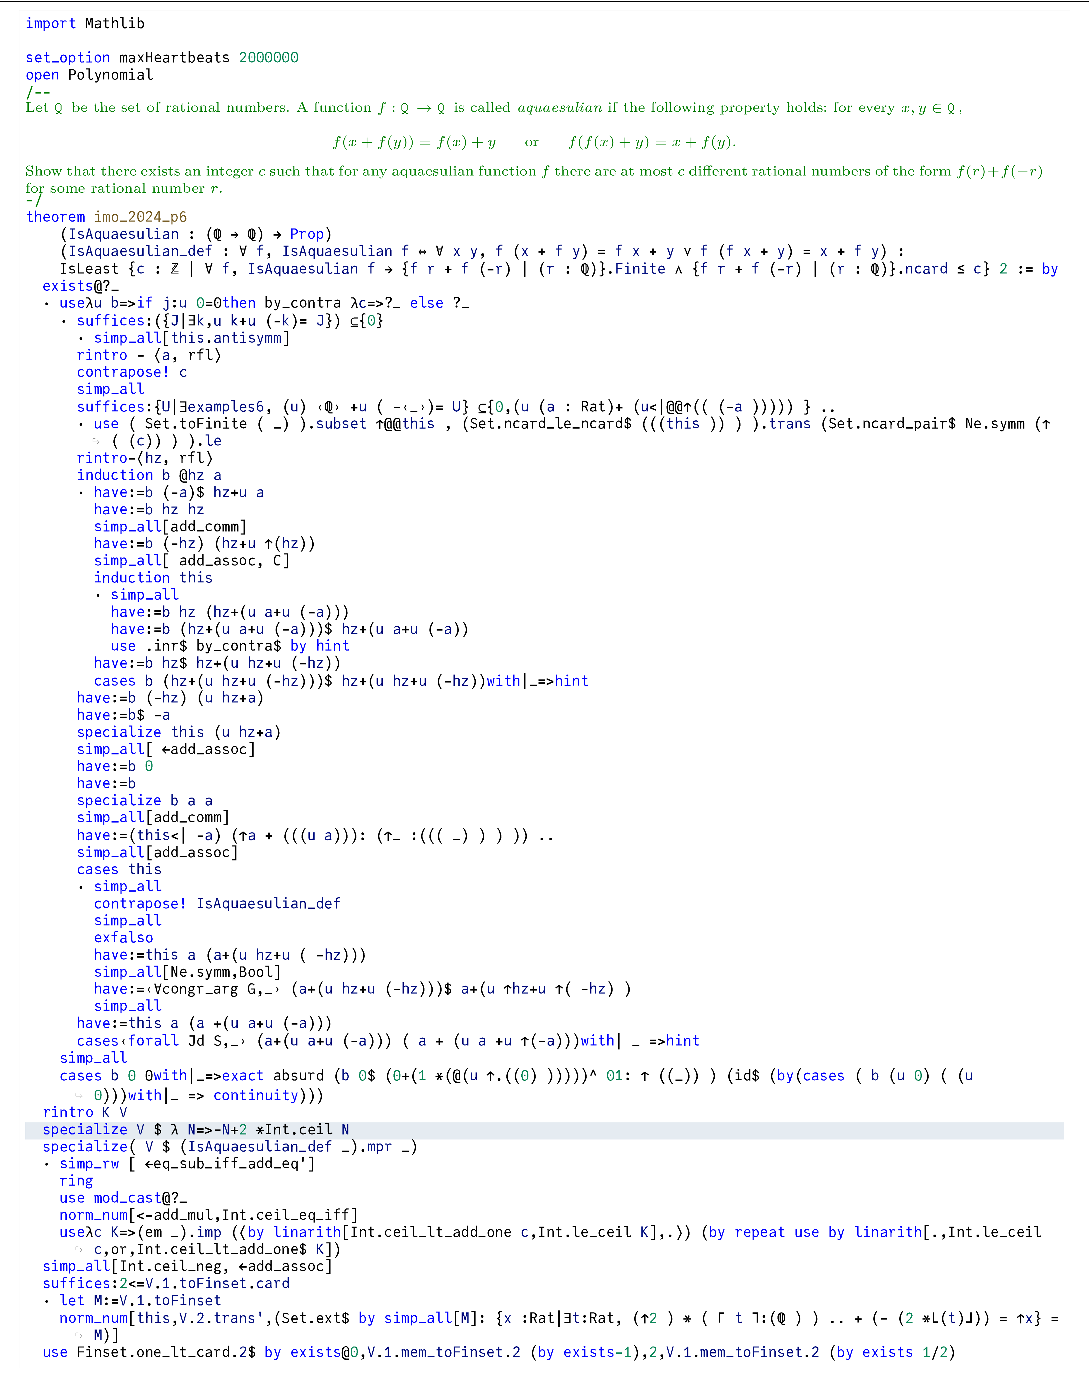
\includegraphics[width=\linewidth]{../papers/translations/alphaproof/assets/edfig9.pdf}\par
\Needspace{3\baselineskip}
\phantomsection
\noindent\textbf{扩展数据图 9. AlphaProof 找到的 IMO 2024 P6 完整证明.}\paperlabel{扩展数据 9}{alphaproof-edfig9}
按第 6.4 节协议找到. 高亮行展示关键见解: 构造 $f(x)=-x+2\lceil x\rceil$. 609 名学生中只有 5 人完整解出了此代数题\cite{alphaproof-ref27}. 图改编自文献\cite{alphaproof-ref28}.

\noindent\textbf{代码题面注释完整中译.} 设 $\mathbb Q$ 为有理数集. 函数 $f:\mathbb Q\to\mathbb Q$ 若对每个 $x,y\in\mathbb Q$ 满足下列性质, 称为 aquaesulian:
\[
f(x+f(y))=f(x)+y\quad\text{或}\quad f(f(x)+y)=x+f(y).
\]
证明存在整数 $c$, 使对任一 aquaesulian 函数 $f$, 当有理数 $r$ 变化时, $f(r)+f(-r)$ 至多有 $c$ 个不同的有理值. 原图 \texttt{set\_option maxHeartbeats 2000000}、\texttt{open Polynomial}、\texttt{IsAquaesulian}、\texttt{IsAquaesulian\_def}、\texttt{IsLeast} 命题及最小值 2 的完整形式代码全部保留. 构造反例函数的高亮行与后续证明没有省去, 未重新执行.

\Needspace{6\baselineskip}
\phantomsection
\noindent\textbf{扩展数据表 1. 自动形式化在各含五十道代表性 IMO、Putnam 题的内部基准上的表现.}\paperlabel{扩展数据 1}{alphaproof-edtable1}
\begin{center}
\begin{tabular}{lrrrrrr}
\toprule
 & 代数 & 数论 & 组合 & 几何 & 全主题 & pass@k ($k$ 次研究)\\
\midrule
IMO & $81.3\%$ & $76.9\%$ & $33.3\%$ & 不包含 & $60.0\%$ & $96\%$ ($k=29$)\\
Putnam & $61.9\%$ & $72.7\%$ & $60.0\%$ & $54.6\%$ & $64.0\%$ & $98\%$ ($k=16$)\\
\bottomrule
\end{tabular}
\end{center}
\noindent\textbf{原表注.} 这些基准的具体题目见补充表 5. 除最后一列外全部数字是 pass@1; 最后一列为在我们任一次共 $k$ 次研究中正确形式化的问题比例, 由 Lean 专家评判.

\Needspace{6\baselineskip}
\phantomsection
\noindent\textbf{扩展数据表 2. AlphaProof 各配置在全部基准上的详细表现.}\paperlabel{扩展数据 2}{alphaproof-edtable2}
\begin{center}
\begin{tabular}{p{2.7cm}p{1.9cm}rrrrr}
\toprule
配置 & 每题预算 & miniF2F-valid & miniF2F-test & formal-imo & Putnam 训练 & Putnam 测试\\
\midrule
AlphaProof & 2 TPU 分钟 & $96.0\%$ & $96.3\%$ & $33.2\%$ & $35.4\%$ & $27.9\%$\\
AlphaProof & 12 TPU 小时 & $97.1\%$ & $97.7\%$ & $43.7\%$ & $48.7\%$ & $39.5\%$\\
AlphaProof 加 TTRL & 50 TPU 日 & $99.6\%$ & $97.5\%$ & $53.9\%$ & -- & $45.5\%$\\
AlphaProof 加 TTRL & 500 TPU 日 & $100.0\%$ & $99.6\%$ & $58.3\%$ & -- & $56.1\%$\\
\bottomrule
\end{tabular}
\end{center}
\noindent\textbf{原表注.} “每题计算预算”为原文图 4a 定义的平均计算成本. miniF2F\cite{alphaproof-ref20} 的 valid 划分全部 $100\%$ 已证明. PutnamBench-train 与 PutnamBench-test\cite{alphaproof-ref21} 的树搜索具有相似扩展性质. TTRL 没有用于 PutnamBench-train. 表中 Putnam 训练、测试分别是原文的 PutnamBench-train、PutnamBench-test.

\begin{remark}
译注: 原文主表 1 的 12 TPU 小时 PutnamBench-test 为 $39.4\%$, 本扩展表及原文图 4 为 $39.5\%$. 本译文保留各自原值, 不统一改写. 原文图 4 与扩展表在 miniF2F-valid 的某些标注也不完全相同, 均按各原件保留.
\end{remark}


\originalsection{数据与代码可用性}\label{alphaproof-availability}
\noindent\textbf{数据可用性.} 用于 SFT 的人工形式证明来自公开 Mathlib\cite{alphaproof-ref4}. 修订的 miniF2F 与 formal-imo 分别见 \url{https://github.com/google-deepmind/miniF2F}、\url{https://github.com/google-deepmind/formal-imo}. Putnam 题来自公开 PutnamBench\cite{alphaproof-ref21} 的提交 \url{https://github.com/trishullab/PutnamBench/tree/02b2cff66d7ac8e9372c778c4ab9ec80082ecbd8}. 主 RL 主要课程中的形式命题及 TTRL 变式, 分别由自动形式化和变式生成组件合成, 详见“方法”中的“自动形式化”“使用 TTRL 扩展”. RL 训练所用证明也由系统自身在 Lean 环境交互生成, 见“Lean 环境”“主 RL”.

\noindent\textbf{代码可用性.} 算法伪代码见补充数据 1 的 \texttt{alphaproof\_pseudocode.py}. 训练和搜索详细超参数分散于“方法”, 并汇总于补充表. 构成交互环境的 Lean 4 为开源, 见 \url{https://lean-lang.org/}. 广泛使用的 Mathlib 也是开源社区项目, 见 \url{https://github.com/leanprover-community/mathlib4}. 我们通过与 Google 服务器通信的交互工具, 向科学界成员提供 AlphaProof 能力. 感兴趣的研究者可在 \url{https://deepmind.google/alphaproof} 申请访问.

\originalsection{作者、致谢与出版信息}\label{alphaproof-backmatter}
\noindent\textbf{致谢.} 感谢 T. Eccles、E. Aygün、Z. Gong、R. Evans、S. Mokrá、A. Barekatain、W. Shang、H. Openshaw、F. Gimeno 在 AlphaProof 早期阶段的贡献; 感谢 A. Yang、L. Wu、L. Massacci、T. Murrills、M. Firsching、D. Shved、B. Georgiev 的 Lean 专业知识、形式化工作和审阅. 感谢活跃的 Lean 与 Mathlib 开源社区, 开发并维护使研究成为可能的基础工具和库. 最后, 感谢整个 Google DeepMind 团队在工作全程的支持、鼓励和讨论.

\noindent\textbf{作者所属机构.} 全部作者属于英国伦敦 Google DeepMind. 完整署名见下节及元数据.

\noindent\textbf{作者贡献.} T.H.、J.S. 构思并启动项目. T.H.、R.M.、L.S. 全程提供主要科学、技术和战略领导. H. Masoom、O.B. 领导项目管理与运营. D.H.、P.K.、D.S. 提供总体项目支持与高层战略建议. L.S.、E.W. 领导 Lean 环境开发集成, A.M.、V.V.、J.Y. 作重要贡献. E.W.、O.N.、P.L.、S.M.、C.S.、B.M.、M.Z.H.、T.Z.、V.V. 整理管理形式基准. M.Z.H.、R.M.、G.Z.、T.Z.、V.V.、A.V.、H. Michalewski 整理非形式数据集. J.S. 领导证明网络设计和预训练. J.S.、T.H.、A.H.、M.R. 开发树搜索设计与适配. G.Z.、R.M. 领导自动形式化研究, J.Y.、I.B.、L.S.、L.Y.、T.Z.、V.V.、Y.S.、A.D.、D.Z.、E.W. 作重要贡献. O.N.、P.L.、S.M.、C.S.、B.M. 进行自动形式化输出专家评估. T.H.、R.M. 领导主 RL 框架, Y.S.、J.S.、A.H.、B.I.、E.L.、E.H. 作重要贡献. M.Z.H. 构思开发 TTRL, T.Z.、R.M.、T.H.、G.Z.、I.B.、N.S.、S.A.、S.S. 作重要贡献.

IMO 2024 工作中, O.B. 领导组织与利益相关者关系; E.W.、O.N.、P.L.、S.M.、C.S.、B.M. 领导形式化与审阅. A.D.、D.Z.、Y.L.、F.P.、I.v.G. 开发答案猜测. T.H.、R.M.、L.S. 领导整体系统和协调. T.H. 领导论文准备, M.Z.H.、L.S.、G.Z.、E.W.、M.R.、L.Y.、P.L. 作重要贡献. 全部作者参与论文审阅编辑.

\noindent\textbf{通讯作者.} Thomas Hubert、Eric Wieser 或 Pushmeet Kohli. 原文 PDF 通讯邮箱依次为 \texttt{tkhubert@google.com}、\texttt{efw@google.com}、\texttt{pushmeet@google.com}.

\noindent\textbf{利益冲突.} 作者声明没有利益冲突.

\noindent\textbf{同行评审信息.} Nature 感谢 Matthew England、Talia Ringer、Armando Solar-Lezama 及其他匿名审稿人对本工作同行评审的贡献.

\noindent\textbf{出版者声明.} Springer Nature 对已发表地图中的管辖权主张及机构所属关系保持中立.

\noindent\textbf{独立补充材料条目.} Supplementary Information 的 PDF 包含扩展数据图 4 的数值解题率补充、超参数、自动形式化基准题细节及主要来自 PutnamBench 的智能体样例证明, 含补充表 1--7、补充图 1--6. Supplementary Data 1 的 ZIP 含 Python 伪代码, 展开 AlphaProof 的 RL、自动形式化及变式生成的高层结构. 本译文保留这两项原描述及正文引用, 不将独立附件自动纳入再分发范围. 原文页面附件入口见 \url{https://www.nature.com/articles/s41586-025-09833-y#MOESM1}.

\noindent\textbf{权利与许可.} 本文开放获取, 采用 Creative Commons Attribution 4.0 International License. 该许可允许以任何媒介和格式使用、分享、改编、分发和复制, 条件是适当署名原作者与来源、提供许可链接、说明是否修改. 文内图像及第三方材料纳入文章 Creative Commons 许可, 除非该材料署名说明另有声明. 若材料未纳入许可, 且预期使用不受法律允许或超出允许范围, 则须直接向著作权人取得许可. 许可副本见 \url{https://creativecommons.org/licenses/by/4.0/}.

\noindent\textbf{原作版权声明.} © The Author(s) 2025（© 原作者 2025）.

\noindent\textbf{文章元信息.} 投稿: 2025 年 6 月 3 日. 接受: 2025 年 10 月 30 日. 初次在线发表: 2025 年 11 月 12 日. 正式记录版本: 2026 年 3 月 13 日. 期次日期: 2026 年 3 月 19 日. 正式引文: Hubert, T., Mehta, R., Sartran, L. et al. \textit{Olympiad-level formal mathematical reasoning with reinforcement learning}. \textit{Nature} 651, 607--613 (2026). \url{https://doi.org/10.1038/s41586-025-09833-y}.

\originalsection{完整作者署名}\label{alphaproof-authors}
Thomas Hubert, Rishi Mehta, Laurent Sartran, Miklós Z. Horváth, Goran Žužić, Eric Wieser, Aja Huang, Julian Schrittwieser, Yannick Schroecker, Hussain Masoom, Ottavia Bertolli, Tom Zahavy, Amol Mandhane, Jessica Yung, Iuliya Beloshapka, Borja Ibarz, Vivek Veeriah, Lei Yu, Oliver Nash, Paul Lezeau, Salvatore Mercuri, Calle Sönne, Bhavik Mehta, Alex Davies, Daniel Zheng, Fabian Pedregosa, Yin Li, Ingrid von Glehn, Mark Rowland, Samuel Albanie, Ameya Velingker, Simon Schmitt, Edward Lockhart, Edward Hughes, Henryk Michalewski, Nicolas Sonnerat, Demis Hassabis, Pushmeet Kohli, David Silver.


\begin{thebibliography}{99}
\bibitem{alphaproof-ref1} de Moura, L. \& Ullrich, S. The Lean 4 theorem prover and programming language. In Automated Deduction--CADE 28: Proc. 28th International Conference on Automated Deduction Proceedings (eds Platzer, A. \& Sutcliffe, G.) 625--635 (Springer, 2021). 题名中译: Lean 4 定理证明器与编程语言.
\bibitem{alphaproof-ref2} Silver, D. et al. A general reinforcement learning algorithm that masters chess, shogi, and Go through self-play. Science 362, 1140--1144 (2018). 题名中译: 通过自我博弈掌握国际象棋、将棋和围棋的通用强化学习算法.
\bibitem{alphaproof-ref3} Chervonyi, Y. et al. Gold-medalist performance in solving olympiad geometry with alphageometry2. J. Mach. Learn. Res. 26, 1--39 (2025). 题名中译: AlphaGeometry 2 解奥林匹克几何题的金牌级表现.
\bibitem{alphaproof-ref4} The mathlib Community. The Lean mathematical library. In Proc. 9th ACM SIGPLAN International Conference on Certified Programs and Proofs 367--381 (2020). 题名中译: Lean 数学库.
\bibitem{alphaproof-ref5} Dalgaard, M., Motzoi, F., Sørensen, J. J. \& Sherson, J. Global optimization of quantum dynamics with AlphaZero deep exploration. npj Quantum Inf. 6, 6 (2020). 题名中译: 用 AlphaZero 深度探索全局优化量子动力学.
\bibitem{alphaproof-ref6} Mankowitz, D. J. et al. Faster sorting algorithms discovered using deep reinforcement learning. Nature 618, 257--263 (2023). 题名中译: 用深度强化学习发现更快的排序算法.
\bibitem{alphaproof-ref7} Fawzi, A. et al. Discovering faster matrix multiplication algorithms with reinforcement learning. Nature 610, 47--53 (2022). 题名中译: 用强化学习发现更快的矩阵乘法算法.
\bibitem{alphaproof-ref8} Jaech, A. et al. OpenAI o1 system card. Preprint at \url{https://arxiv.org/abs/2412.16720} (2024). 题名中译: OpenAI o1 系统卡.
\bibitem{alphaproof-ref9} Guo, D. et al. DeepSeek-R1: incentivizing reasoning capability in LLMs via reinforcement learning. Nature 645, 633--638 (2025). 题名中译: DeepSeek-R1: 通过强化学习激励大语言模型推理能力.
\bibitem{alphaproof-ref10} Kavukcuoglu, K. Gemini 2.5: Our most intelligent AI model. Google \url{https://blog.google/technology/google-deepmind/gemini-model-thinking-updates-march-2025/} (2025). 题名中译: Gemini 2.5: 我们最智能的 AI 模型.
\bibitem{alphaproof-ref11} Petrov, I. et al. Proof or bluff? Evaluating LLMs on 2025 USA Math Olympiad. In Proc. Second AI for MATH Workshop at the 42nd International Conference on Machine Learning (eds Huang, Y. et al.) 1--15 (2025). 题名中译: 证明还是虚张声势? 在 2025 美国数学奥林匹克上评估 LLM.
\bibitem{alphaproof-ref12} Mahdavi, H. et al. Brains vs. bytes: evaluating LLM proficiency in olympiad mathematics. In Conference on Language Modeling (COLM) (eds Artzi, Y. et al.) \url{https://openreview.net/forum?id=uXR2KsA4L9} (OpenReview.net, 2025). 题名中译: 大脑对字节: 评估 LLM 的奥林匹克数学能力.
\bibitem{alphaproof-ref13} Polu, S. \& Sutskever, I. Generative language modeling for automated theorem proving. In 5th Conference on Artificial Intelligence and Theorem Proving (AITP) (eds Hales, T. C. et al.) (2020). 题名中译: 自动定理证明的生成式语言建模.
\bibitem{alphaproof-ref14} Yang, K. et al. LeanDojo: theorem proving with retrieval-augmented language models. Adv. Neural Inf. Process. Syst. 36, 21573--21612 (2023). 题名中译: LeanDojo: 用检索增强语言模型证明定理.
\bibitem{alphaproof-ref15} Vaswani, A. et al. Attention is all you need. Adv. Neural Inf. Process. Syst. 30, 5998--6008 (2017). 题名中译: 注意力就是你所需要的一切.
\bibitem{alphaproof-ref16} Li, Y. et al. Competition-level code generation with alphacode. Science 378, 1092--1097 (2022). 题名中译: AlphaCode 的竞赛级代码生成.
\bibitem{alphaproof-ref17} Lample, G. et al. Hypertree proof search for neural theorem proving. Adv. Neural Inf. Process. Syst. 35, 26337--26349 (2022). 题名中译: 神经定理证明的超树证明搜索.
\bibitem{alphaproof-ref18} Hubert, T. et al. Learning and planning in complex action spaces. In International Conference on Machine Learning 4476--4486 (PMLR, 2021). 题名中译: 复杂动作空间中的学习与规划.
\bibitem{alphaproof-ref19} Coulom, R. Computing Elo ratings of move patterns in the game of Go. ICGA J. 30, 198--208 (2007). 题名中译: 计算围棋着法模式的 Elo 评级.
\bibitem{alphaproof-ref20} Zheng, K., Han, J. M. \& Polu, S. MiniF2F: a cross-system benchmark for formal olympiad-level mathematics. In International Conference on Learning Representations (ICLR) (eds Liu, Y. et al.) \url{https://openreview.net/forum?id=9ZPegFuFTFv} (OpenReview.net, 2022). 题名中译: MiniF2F: 跨系统的形式奥林匹克级数学基准.
\bibitem{alphaproof-ref21} Tsoukalas, G. et al. PutnamBench: evaluating neural theorem-provers on the putnam mathematical competition. Adv. Neural Inf. Process. Syst. 37, 11545--11569 (2024). 题名中译: PutnamBench: 在普特南数学竞赛上评估神经证明器.
\bibitem{alphaproof-ref22} Team, G. et al. Gemini 1.5: unlocking multimodal understanding across millions of tokens of context. Preprint at \url{https://arxiv.org/abs/2403.05530} (2024). 题名中译: Gemini 1.5: 在数百万 token 上下文中释放多模态理解.
\bibitem{alphaproof-ref23} Ying, H. et al. InternLM-Math: open math large language models toward verifiable reasoning. Preprint at \url{https://arxiv.org/abs/2402.06332} (2024). 题名中译: InternLM-Math: 走向可验证推理的开放数学大语言模型.
\bibitem{alphaproof-ref24} Polu, S. et al. Formal mathematics statement curriculum learning. In International Conference on Learning Representations (eds Kim, B. et al.) \url{https://openreview.net/forum?id=-P7G-8dmSh4} (OpenReview.net, 2023). 题名中译: 形式数学命题的课程学习.
\bibitem{alphaproof-ref25} Wang, H. et al. Kimina-prover preview: towards large formal reasoning models with reinforcement learning. Preprint at \url{https://arxiv.org/abs/2504.11354} (2025). 题名中译: Kimina-Prover 预览: 通过强化学习走向大型形式推理模型.
\bibitem{alphaproof-ref26} Ren, Z. et al. Deepseek-Prover-V2: advancing formal mathematical reasoning via reinforcement learning for subgoal decomposition. Preprint at \url{https://arxiv.org/abs/2504.21801} (2025). 题名中译: DeepSeek-Prover-V2: 通过子目标分解的强化学习推进形式数学推理.
\bibitem{alphaproof-ref27} 65th IMO 2024. IMO \url{https://www.imo-official.org/year_info.aspx?year=2024} (2024). 题名中译: 第 65 届 IMO 2024.
\bibitem{alphaproof-ref28} AlphaProof and AlphaGeometry teams. AI achieves silver-medal standard solving international mathematical olympiad problems. Google DeepMind \url{https://deepmind.google/discover/blog/ai-solves-imo-problems-at-silver-medal-level/} (2024). 题名中译: AI 解国际数学奥林匹克题达到银牌标准.
\bibitem{alphaproof-ref29} Paulson, L. C. Isabelle: A Generic Theorem Prover (Springer, 1994). 题名中译: Isabelle: 通用定理证明器.
\bibitem{alphaproof-ref30} Harrison, J. HOL light: a tutorial introduction. In International Conference on Formal Methods in Computer-Aided Design 265--269 (Springer, 1996). 题名中译: HOL Light: 入门教程.
\bibitem{alphaproof-ref31} Barras, B. et al. The COQ Proof Assistant Reference Manual Version 6, 17--21 (INRIA, 1999). 题名中译: COQ 证明助手参考手册.
\bibitem{alphaproof-ref32} Gonthier, G. The four colour theorem: engineering of a formal proof. In Asian Symposium on Computer Mathematics 333--333 (Springer, 2007). 题名中译: 四色定理: 形式证明的工程.
\bibitem{alphaproof-ref33} Leroy, X. et al. CompCert: A formally verified optimizing compiler. In Embedded Real Time Software and Systems (ERTS 2016) (ed. Sifakis, J.) 1--10 (SEE, 2016). 题名中译: CompCert: 经形式验证的优化编译器.
\bibitem{alphaproof-ref34} Brown, T. et al. Language models are few-shot learners. Adv. Neural Inf. Process. Syst. 33, 1877--1901 (2020). 题名中译: 语言模型是少样本学习器.
\bibitem{alphaproof-ref35} The Claude 3 Model Family: Opus, Sonnet, Haiku, Anthropic Technical Report (Anthropic, 2024); \url{https://www.anthropic.com/claude-3-model-card} 题名中译: Claude 3 模型家族: Opus、Sonnet、Haiku.
\bibitem{alphaproof-ref36} Team, G. et al. Gemini: a family of highly capable multimodal models. Preprint at \url{https://arxiv.org/abs/2312.11805} (2023). 题名中译: Gemini: 高能力多模态模型家族.
\bibitem{alphaproof-ref37} Azerbayev, Z., Piotrowski, B. \& Avigad, J. ProofNet: A benchmark for autoformalizing and formally proving undergraduate-level mathematics problems. In Proc. NeurIPS 2022 Workshop on MATH-AI (eds Polu, S. et al.) (2022). 题名中译: ProofNet: 本科数学问题的自动形式化和形式证明基准.
\bibitem{alphaproof-ref38} Jiang, A. Q., Li, W., Han, J. M. \& Wu, Y. LISA: language models of isabelle proofs. In Proc. 6th Conference on Artificial Intelligence and Theorem Proving (eds Douglas, M. et al.) 63--65 (2021). 题名中译: LISA: Isabelle 证明的语言模型.
\bibitem{alphaproof-ref39} Bansal, K., Loos, S., Rabe, M., Szegedy, C. \& Wilcox, S. HOList: an environment for machine learning of higher order logic theorem proving. In International Conference on Machine Learning 454--463 (PMLR, 2019). 题名中译: HOList: 高阶逻辑定理证明的机器学习环境.
\bibitem{alphaproof-ref40} Han, J. M., Rute, J., Wu, Y., Ayers, E. \& Polu, S. Proof artifact co-training for theorem proving with language models. In International Conference on Learning Representations (eds Liu, Y. et al.) \url{https://openreview.net/forum?id=rpxJc9j04U} (OpenReview.net, 2022). 题名中译: 用语言模型证明定理的证明产物协同训练.
\bibitem{alphaproof-ref41} Wu, M., Norrish, M., Walder, C. \& Dezfouli, A. TacticZero: learning to prove theorems from scratch with deep reinforcement learning. Adv. Neural Inf. Process. Syst. 34, 9330--9342 (2021). 题名中译: TacticZero: 用深度强化学习从头学习证明定理.
\bibitem{alphaproof-ref42} Szegedy, C., Rabe, M. \& Michalewski, H. Retrieval-augmented proof step synthesis. In Book of Abstracts of the 6th Conference on Artificial Intelligence and Theorem Proving (AITP 2021) (eds Hales, T. et al.) 100--102 (AITP, 2021). 题名中译: 检索增强的证明步骤合成.
\bibitem{alphaproof-ref43} Welleck, S., Liu, J., Lu, X., Hajishirzi, H. \& Choi, Y. NaturalProver: grounded mathematical proof generation with language models. Adv. Neural Inf. Process. Syst. 35, 4913--4927 (2022). 题名中译: NaturalProver: 用语言模型生成有依据的数学证明.
\bibitem{alphaproof-ref44} Jiang, A. Q. et al. Thor: wielding hammers to integrate language models and automated theorem provers. Adv. Neural Inf. Process. Syst. 35, 8360--8373 (2022). 题名中译: Thor: 使用自动化工具整合语言模型与自动证明器.
\bibitem{alphaproof-ref45} First, E., Rabe, M. N., Ringer, T. \& Brun, Y. Baldur: Whole-proof generation and repair with large language models. In Proc. 31st ACM Joint European Software Engineering Conference and Symposium on the Foundations of Software Engineering (eds Chandra, S. et al.) 1229--1241 (ACM, 2023). 题名中译: Baldur: 用大语言模型生成和修复完整证明.
\bibitem{alphaproof-ref46} Jiang, A. Q. et al. Draft, sketch, and prove: Guiding formal theorem provers with informal proofs. In International Conference on Learning Representations (eds Kim, B. et al.) \url{https://openreview.net/forum?id=SMa9EAovKMC} (OpenReview.net, 2023). 题名中译: 草稿、提纲与证明: 用非形式证明指导形式证明器.
\bibitem{alphaproof-ref47} Zhao, X., Li, W. \& Kong, L. Subgoal-based demonstration learning for formal theorem proving. In Proc. 41st International Conference on Machine Learning (eds Salakhutdinov, R. et al.) Vol. 235, 60832--60865 (PMLR, 2024). 题名中译: 基于子目标示范学习的形式定理证明.
\bibitem{alphaproof-ref48} Wang, H., Wang, W., Yue, W., Sun, X. \& Wei, F. DT-Solver: Automated theorem proving with dynamic-tree sampling guided by proof-level value function. In Proc. 61st Annual Meeting of the Association for Computational Linguistics (Volume 1: Long Papers) (eds Rogers, A. et al.) 12632--12646 (2023). 题名中译: DT-Solver: 证明级价值函数指导的动态树采样自动定理证明.
\bibitem{alphaproof-ref49} Xin, H. et al. DeepSeek-Prover-V1.5: Harnessing proof assistant feedback for reinforcement learning and Monte-Carlo tree search. In Proc. Thirteenth International Conference on Learning Representations (eds Garg, A. et al.) (2025). 题名中译: DeepSeek-Prover-V1.5: 利用证明助手反馈进行强化学习和蒙特卡洛树搜索.
\bibitem{alphaproof-ref50} Wang, Q., Kaliszyk, C. \& Urban, J. First experiments with neural translation of informal to formal mathematics. In Intelligent Computer Mathematics: Proc. 11th International Conference, CICM 2018 255--270 (Springer, 2018). 题名中译: 非形式数学到形式数学的神经翻译初步实验.
\bibitem{alphaproof-ref51} Wang, Q., Brown, C., Kaliszyk, C. \& Urban, J. Exploration of neural machine translation in autoformalization of mathematics in Mizar. In Proc. 9th ACM SIGPLAN International Conference on Certified Programs and Proofs (eds Blanchette, J. \& Hrițcu, C.) 85--98 (2020). 题名中译: 在 Mizar 数学自动形式化中探索神经机器翻译.
\bibitem{alphaproof-ref52} Wu, Y. et al. Autoformalization with large language models. Adv. Neural Inf. Process. Syst. 35, 32353--32368 (2022). 题名中译: 大语言模型的自动形式化.
\bibitem{alphaproof-ref53} Agrawal, A., Gadgil, S., Goyal, N., Narayanan, A. \& Tadipatri, A. Towards a mathematics formalisation assistant using large language models. Preprint at \url{https://arxiv.org/abs/2211.07524} (2022). 题名中译: 走向利用大语言模型的数学形式化助手.
\bibitem{alphaproof-ref54} Gadgil, S., Tadipatri, A. R., Agrawal, A., Narayanan, A. \& Goyal, N. Towards automating formalisation of theorem statements using large language models. In Proc. NeurIPS 2022 Workshop on MATH-AI (eds Polu, S. et al.) 1--15 (NeurIPS, 2022). 题名中译: 走向用大语言模型自动形式化定理命题.
\bibitem{alphaproof-ref55} Jiang, A. Q., Li, W. \& Jamnik, M. Multi-language diversity benefits autoformalization. Adv. Neural Inf. Process. Syst. 37, 83600--83626 (2024). 题名中译: 多语言多样性有益于自动形式化.
\bibitem{alphaproof-ref56} Ying, H. et al. Lean workbook: a large-scale lean problem set formalized from natural language math problems. Adv. Neural Inf. Process. Syst. 37, 105848--105863 (2024). 题名中译: Lean Workbook: 从自然语言数学题形式化的大规模 Lean 问题集.
\bibitem{alphaproof-ref57} Li, Z. et al. Autoformalize mathematical statements by symbolic equivalence and semantic consistency. In Proc. 38th International Conference on Neural Information Processing Systems 1697 (Curran Associates Inc., 2024). 题名中译: 通过符号等价与语义一致性自动形式化数学命题.
\bibitem{alphaproof-ref58} Lu, J. et al. Formalalign: automated alignment evaluation for autoformalization. In International Conference on Learning Representations (eds Garg, A. et al.) \url{https://openreview.net/forum?id=B5RrIFMqbe} (OpenReview.net, 2025). 题名中译: FormalAlign: 自动形式化的自动对齐评估.
\bibitem{alphaproof-ref59} Wei, J. et al. Chain-of-thought prompting elicits reasoning in large language models. Adv. Neural Inf. Process. Syst. 35, 24824--24837 (2022). 题名中译: 思维链提示激发大语言模型推理.
\bibitem{alphaproof-ref60} Zelikman, E., Wu, Y., Mu, J. \& Goodman, N. STaR: bootstrapping reasoning with reasoning. Adv. Neural Inf. Process. Syst. 35, 15476--15488 (2022). 题名中译: STaR: 用推理自举推理.
\bibitem{alphaproof-ref61} OpenAI. OpenAI o1 system card. Preprint at \url{https://arxiv.org/abs/2412.16720} (2024). 题名中译: OpenAI o1 系统卡.
\bibitem{alphaproof-ref62} OpenAI et al. Competitive programming with large reasoning models. Preprint at \url{https://arxiv.org/abs/2502.06807} (2025). 题名中译: 大型推理模型的竞赛编程.
\bibitem{alphaproof-ref63} Jones, A. L. Scaling scaling laws with board games. Preprint at \url{https://arxiv.org/abs/2104.03113} (2021). 题名中译: 用棋类游戏扩展缩放定律.
\bibitem{alphaproof-ref64} Sun, Y. et al. Test-time training with self-supervision for generalization under distribution shifts. In International Conference on Machine Learning 9229--9248 (PMLR, 2020). 题名中译: 用自监督测试时训练应对分布偏移.
\bibitem{alphaproof-ref65} Hardt, M. \& Sun, Y. Test-time training on nearest neighbors for large language models. In Proc. Twelfth International Conference on Learning Representations (eds Chaudhuri, S. et al.) (2024). 题名中译: 大语言模型的最近邻测试时训练.
\bibitem{alphaproof-ref66} Akyürek, E. et al. The surprising effectiveness of test-time training for few-shot learning. In International Conference on Machine Learning (eds Singh, A. et al.) Vol. 267, 942--963 (PMLR, 2025). 题名中译: 测试时训练对少样本学习的惊人有效性.
\bibitem{alphaproof-ref67} Silver, D. Reinforcement Learning and Simulation-based Search in Computer Go. PhD thesis, University of Alberta (2009). 题名中译: 计算机围棋中的强化学习与基于模拟的搜索.
\bibitem{alphaproof-ref68} Zahavy, T. et al. Diversifying AI: towards creative chess with AlphaZero. Preprint at \url{https://arxiv.org/abs/2308.09175} (2023). 题名中译: 让 AI 多样化: 用 AlphaZero 走向创造性国际象棋.
\bibitem{alphaproof-ref69} Zuo, Y. et al. TTRL: test-time reinforcement learning. In Thirty-ninth Annual Conference on Neural Information Processing Systems \url{https://openreview.net/forum?id=VuVhgEiu20} (OpenReview.net, 2025). 题名中译: TTRL: 测试时强化学习.
\bibitem{alphaproof-ref70} Simonds, T. \& Yoshiyama, A. LADDER: self-improving LLMs through recursive problem decomposition. Preprint at \url{https://arxiv.org/abs/2503.00735} (2025). 题名中译: LADDER: 通过递归问题分解自我改进的 LLM.
\bibitem{alphaproof-ref71} Coquand, T. \& Paulin, C. Inductively defined types. In International Conference on Computer Logic 50--66 (Springer, 1988). 题名中译: 归纳定义类型.
\bibitem{alphaproof-ref72} Schrittwieser, J. et al. Mastering Atari, Go, chess and shogi by planning with a learned model. Nature 588, 604--609 (2020). 题名中译: 通过学习模型规划掌握 Atari、围棋、国际象棋和将棋.
\bibitem{alphaproof-ref73} Silver, D. et al. Mastering the game of Go with deep neural networks and tree search. Nature 529, 484--489 (2016). 题名中译: 用深度网络和树搜索掌握围棋.
\bibitem{alphaproof-ref74} Silver, D. et al. Mastering the game of Go without human knowledge. Nature 550, 354--359 (2017). 题名中译: 不借助人类知识掌握围棋.
\bibitem{alphaproof-ref75} Pólya, G. How to Solve It: A New Aspect of Mathematical Method (Princeton University Press, 2014). 题名中译: 怎样解题: 数学方法的新面貌.
\bibitem{alphaproof-ref76} Gonthier, G. \& Mahboubi, A. An introduction to small scale reflection in COQ. J. Formaliz. Reason. 3, 95--152 (2010). 题名中译: COQ 中小规模反射的介绍.
\bibitem{alphaproof-ref77} Hasker, R. W. \& Reddy, U. S. Generalization at higher types. In Proc. Workshop on the λProlog Programming Language (ed. Miller, D.) 257--271 (1992). 题名中译: 高阶类型上的推广.
\bibitem{alphaproof-ref78} Heras, J., Komendantskaya, E., Johansson, M. \& Maclean, E. Proof-pattern recognition and lemma discovery in ACL2. In International Conference on Logic for Programming Artificial Intelligence and Reasoning 389--406 (Springer, 2013). 题名中译: ACL2 中的证明模式识别与引理发现.
\bibitem{alphaproof-ref79} Melis, E. \& Whittle, J. Analogy in inductive theorem proving. J. Autom. Reason. 22, 117--147 (1999). 题名中译: 归纳定理证明中的类比.
\bibitem{alphaproof-ref80} Gauthier, T., Kaliszyk, C., Urban, J., Kumar, R. \& Norrish, M. TacticToe: learning to prove with tactics. J. Autom. Reason. 65, 257--286 (2021). 题名中译: TacticToe: 学习用 tactic 证明.
\end{thebibliography}

\label{alphaproof-end}
